\documentclass{article}
\usepackage{NotesPackage}
\usepackage{csquotes}
\usepackage[justification=centering]{caption}
\usepackage[section]{placeins}  % make all figures show before the start of the next section

\counterwithin{figure}{section}
\counterwithin{table}{section}
\counterwithin{equation}{section}

\title{Fluid Mechanics}
\date{September 16, 2019}
\author{Willoughby Seago}

\newcommand{\notesVersion}{1.0}
\newcommand{\notesDate}{04/01/2021}

\begin{document}
    \maketitle
    These are my notes for the \textit{fluid mechanics 2} course from the University of Edinburgh School of Engineering, which I took as an optional course from outside the School of Physics.
    When I took this course in the 2019/20 academic year it was taught by Professor Tom Bruce\footnote{\url{https://www.eng.ed.ac.uk/about/people/prof-tom-bruce}}.
    These notes are based on the lectures delivered as part of this course, and the notes provided as part of this course.
    The content within is correct to the best of my knowledge but if you find a mistake or just disagree with something or think it could be improved please let me know.
    
    These notes were produced using \LaTeX\footnote{\url{https://www.latex-project.org/}}.
    Graphs where plotted using Python\footnote{\url{https://www.python.org/}}, Matplotlib\footnote{\url{https://matplotlib.org/}}, NumPy\footnote{\url{https://numpy.org/}}, and SciPy\footnote{\url{https://scipy.org/scipylib/}}.
    Diagrams were drawn with tikz\footnote{\url{https://www.ctan.org/pkg/pgf}}.
    Some images were taken from the lecture notes provided.
    
    This is version \notesVersion~of these notes, which is up to date as of \notesDate.
    \begin{flushright}
        Willoughby Seago
        
        s1824487@ed.ac.uk
    \end{flushright}
    \clearpage
    \tableofcontents
    \listoffigures
    \listoftables
    \clearpage
    
    \section{Viscosity}
    Definition of a fluid:
    \begin{displayquote}
        Fluids lack ability to offer permanent resistance to a deforming force, They deform continuously for as long as the force is applied
    \end{displayquote}
    Deformation is caused by a shear force (force that acts along the surface). A fluid is at rest if and only if there are no shearing forces (ie all forces are perpendicular to the plane of the surface of the fluid)
    
    Imagine a unit of fluid being deformed by a shear force \(F\) applied to one face of area \(A\) as in the diagram below:
    \begin{center}
        \begin{tikzpicture}
            % \draw[lightgray] (0, 0) grid (10, 10);
            \draw (0, 0) -- (0, 3) -- (4, 3) -- (4, 0) -- cycle;
            \draw[dashed] (0, 0) -- (1, 3);
            \draw[dashed] (4, 3) -- (5, 3);
            \draw[dashed] (4, 0) -- (5, 3);
            \draw[->] (5, 3) -- (6, 3);
            \node[right] at (6, 3) {\(F\)};
            \node at (0.2, 1) {\(\varphi\)};
        \end{tikzpicture}
    \end{center}
    The shear stress \(\tau\) \(\left([\tau] = \si{N.m^{-2}}\right)\) is given by:
    \[\frac{F}{A} = \tau\]
    For a solid \(\varphi \propto \tau\) however for a fluid the rate of change is proportional:
    \[\pdv{\varphi}{t} \propto \tau\]
    We can approximate \(\varphi\) as below
    \begin{center}
        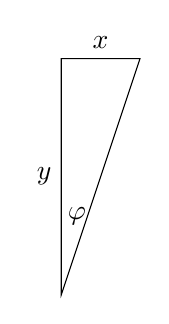
\begin{tikzpicture}
            \draw (0, 0) -- (0, 3) -- (1, 3) -- cycle;
            \node at (0.2, 1) {\(\varphi\)};
            \node[left] at (0, 1.5) {\(y\)};
            \node[above] at (0.5, 3) {\(x\)};
        \end{tikzpicture}
    \end{center}
    \[\sin\varphi = \frac{x}{y}\approx\varphi\]
    \[\pdv{\varphi}{t} \approx \pdv{t}\left(\frac{x}{y}\right) = \frac{1}{y}\pdv{x}{t}=\frac{u}{y}\propto\tau\]
    where \(u\) is the velocity of the fluid (since all motion is in the \(x\) direction)
    \[\tau=\text{const}\cdot\frac{u}{y}\implies\tau = \mu\dv{u}{y}\]
    We call \(\mu\) the dynamic viscosity, \([\mu] = \si{kg.m^{-1}.s^{-1}}\). This is Newton's law of viscosity.
    
    From this we can see that for the same shear stress \(\tau\) a fluid with a lower viscosity will deform faster. This law only applies to Newtonian fluids.
    
    Shearing forces in the body of the fluid arise due to adjacent layers of fluid moving past each other.
    
    The no-slip condition is that at boundaries the velocity is the same on both sides, that is there is no sliding past each other of the layers.
    \begin{center}
        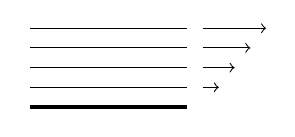
\begin{tikzpicture}
            % boundary
            \draw[ultra thick] (0, 0) -- (2, 0);
            
            % liquid lines
            \draw (0, 0.25) -- (2, 0.25);
            \draw (0, 0.5) -- (2, 0.5);
            \draw (0, 0.75) -- (2, 0.75);
            \draw (0, 1) -- (2, 1);
            
            % arrows
            \draw[->] (2.2, 0.25) -- (2.4, 0.25);
            \draw[->] (2.2, 0.5) -- (2.6, 0.5);
            \draw[->] (2.2, 0.75) -- (2.8, 0.75);
            \draw[->] (2.2, 1) -- (3, 1);
        \end{tikzpicture}
    \end{center}
    Since the boundary is stationary the liquid right next to it must also be stationary. The existence of a velocity gradient like this implies the existence of shear forces.
    The viscosity of a gas \((\mu_\text{gas})\) is much less than the viscosity of a liquid \((\mu_\text{liquid})\). In gasses the viscosity increases as temperature increases as a higher temperature means more collisions so more friction. In a liquid the viscosity decreases as the temperature increases as the particles have more energy to overcome the intermolecular forces that cause the friction that causes the viscosity.
    
    Note that it is common to see the kinematic viscosity \(\nu =\mu/\rho\) where \(\rho\) is the density of the fluid.
    
    \section{Fluid properties}
    Density \(\rho\) is the mass per unit volume, \(\rho = m/V\), \([\rho]=\si{kg.m^{-3}}\).
    
    Specific density or specific gravity is the ratio of the density to that of water, \(\rho/\rho_{\text{water}}=\rho/\SI{1000}{kg.m^{-3}}\).
    
    Flows in which variations in density are negligible are termed incompressible, 
    if instead variations in density are not negligible then the flow is known as compressible
    
    Liquid flows are incompressible. 
    Gas flows in which the speed of flow \(u\) is much less than the speed of sound in the fluid \(c_s\) may also be regarded as incompressible.
    We can define Mach number \(M = u/c_s\). For \(M\le\sim0.3\) we have \(\Delta\rho/\rho\le\sim\SI{5}{\%}\).
    
    Surface tension \(\sigma\) is the force in a liquids surface along lines of unit length in the surface. 
    \(\sigma\) is constant over the surface for a given temperature. 
    As the temperature increases \(\sigma\) decreases.
    The effect of surface tension is to reduce the surface area of the liquid.
    \(\sigma\) is often negligible for low enough surface area to volume ratios.
    This means that \(\sigma\) is most important in high surface area cases such as bubbles, aerosols or films.
    The cause of \(\sigma\) is unbalanced forces in a liquid at the surface:
    \begin{center}
        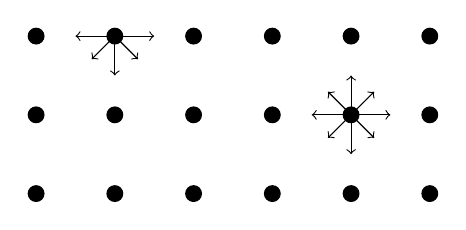
\begin{tikzpicture}
            %\draw[lightgray] (0, 0) grid (5, 3);
            \draw[fill = black] (0, 0) circle (0.1cm);
            \draw[fill = black] (1, 0) circle (0.1cm);
            \draw[fill = black] (2, 0) circle (0.1cm);
            \draw[fill = black] (3, 0) circle (0.1cm);
            \draw[fill = black] (4, 0) circle (0.1cm);
            \draw[fill = black] (5, 0) circle (0.1cm);
            \draw[fill = black] (0, 1) circle (0.1cm);
            \draw[fill = black] (1, 1) circle (0.1cm);
            \draw[fill = black] (2, 1) circle (0.1cm);
            \draw[fill = black] (3, 1) circle (0.1cm);
            \draw[fill = black] (4, 1) circle (0.1cm);
            \draw[fill = black] (5, 1) circle (0.1cm);
            \draw[fill = black] (0, 2) circle (0.1cm);
            \draw[fill = black] (1, 2) circle (0.1cm);
            \draw[fill = black] (2, 2) circle (0.1cm);
            \draw[fill = black] (3, 2) circle (0.1cm);
            \draw[fill = black] (4, 2) circle (0.1cm);
            \draw[fill = black] (5, 2) circle (0.1cm);
            
            \draw[->] (1, 2) -- (1, 1.5);
            \draw[->] (1, 2) -- (0.5, 2);
            \draw[->] (1, 2) -- (1.5, 2);
            \draw[->] (1, 2) -- (0.707, 1.707);
            \draw[->] (1, 2) -- (1.293, 1.707);
            
            \draw[->] (4, 1) -- (4, 0.5);
            \draw[->] (4, 1) -- (3.5, 1);
            \draw[->] (4, 1) -- (4.5, 1);
            \draw[->] (4, 1) -- (4, 1.5);
            \draw[->] (4, 1) -- (3.707, 0.707);
            \draw[->] (4, 1) -- (4.293, 0.707);
            \draw[->] (4, 1) -- (3.707, 1.293);
            \draw[->] (4, 1) -- (4.293, 1.293);
        \end{tikzpicture}
    \end{center}
    
    Laminar flow is characterised by smooth fluid motion in layers. 
    Dye injected into a laminar flow appears as a single line.
    Velocity may differ from layer to layer.
    
    Turbulent flow is characterised by random 3D motion and a mean flow
    \begin{center}
        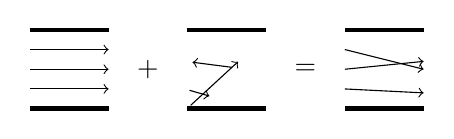
\begin{tikzpicture}
            %\draw[lightgray] (0, 0) grid (5, 2);
            \draw[ultra thick] (0, 0) -- (1, 0);
            \draw[ultra thick] (0, 1) -- (1, 1);
            \draw[ultra thick] (2, 0) -- (3, 0);
            \draw[ultra thick] (2, 1) -- (3, 1);
            \draw[ultra thick] (4, 0) -- (5, 0);
            \draw[ultra thick] (4, 1) -- (5, 1);
            
            \draw[->] (0, 0.75) -- (1, 0.75);
            \draw[->] (0, 0.5) -- (1, 0.5);
            \draw[->] (0, 0.25) -- (1, 0.25);
            
            \draw[->] (2.027, 0.233) -- (2.28, 0.16);
            \draw[->] (2.042, 0.042) -- (2.644, 0.596);
            \draw[->] (2.563, 0.525) -- (2.065, 0.589);

            \draw[->] (4, 0.75) -- (5, 0.5);
            \draw[->] (4, 0.5) -- (5, 0.6);
            \draw[->] (4, 0.25) -- (5, 0.2);
            
            \node at (1.5, 0.5) {\(+\)};
            \node at (3.5, 0.5) {\(=\)};
        \end{tikzpicture}
    \end{center}
    Dye injected into turbulent flow breaks up into lots of entangled threads.
    
    Reynold's number can be calculated for a fluid in a pipe diameter \(D\) as
    \[Re=\frac{\rho u D}{\mu}=\frac{\rho D}{\nu}\]
    For flow in a pipe the Reynold's number can tell us the flow type:
    \begin{center}
        \begin{tabular}{cl}
            \(Re<\sim 2000\) & Laminar flow if undisturbed\\
            \(Re>\sim 4000\) & Turbulent flow\\
            \(2000<Re<4000\) & Transitional flow
        \end{tabular}
    \end{center}
    Transitional flow can be either laminar or turbulent but not both at the same time. It can however switch back and forth between the two flow types.
    
    From this we see that at low Reynold's numbers the viscous forces dominate and higher Reynold's numbers the viscous forces are less important and possibly negligible.
    
    \begin{center}
        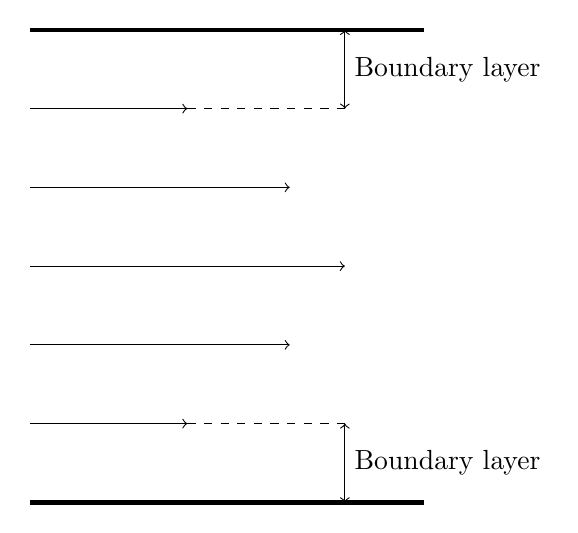
\begin{tikzpicture}
            %\draw[lightgray] (0, 0) grid (6, 6);
            \draw[ultra thick] (0, 0) -- (5, 0);
            \draw[ultra thick] (0, 6) -- (5, 6);
            
            \draw[->] (0, 3) -- (4, 3);
            \draw[->] (0, 2) -- (3.3, 2);
            \draw[->] (0, 4) -- (3.3, 4);
            \draw[->] (0, 1) -- (2, 1);
            \draw[->] (0, 5) -- (2, 5);
            
            \draw[<->] (4, 0) -- (4, 1);
            \draw[dashed] (2, 1) -- (4, 1);
            \node[right] at (4, 0.5) {Boundary layer};
            \draw[<->] (4, 5) -- (4, 6);
            \draw[dashed] (2, 5) -- (4, 5);
            \node[right] at (4, 5.5) {Boundary layer};
        \end{tikzpicture}
    \end{center}
    The velocity profile \(u(y)\) of flow in a pipe describes how the velocity of the fluid changes as you go across the pipe.
    The no slip condition applies at the walls. Because of this the flow near the walls is slow. 
    The region where it is slow is called the boundary layer. 
    The width of the boundary layer is \(\delta\). 
    \(\delta\) increases as viscosity \(\mu\) increases and also as the distance along the pipe increases. 
    \(\delta\) decreases as the free stream (not in boundary layer) speed \(u\) increases.
    
    For laminar flow the velocity profile is parabolic.
    For turbulent flow the velocity profile is much flatter due to effective turbulent mixing across the pipe.
    The no slip condition must still apply but the boundary layer will be much thinner.
    Sometimes it is useful to consider ideal flow which is incompressible, inviscid (no viscous forces) and has a flat velocity profile (note this requires the no slip condition to be broken at the walls).
    
    \begin{figure}[ht]
        \centering
        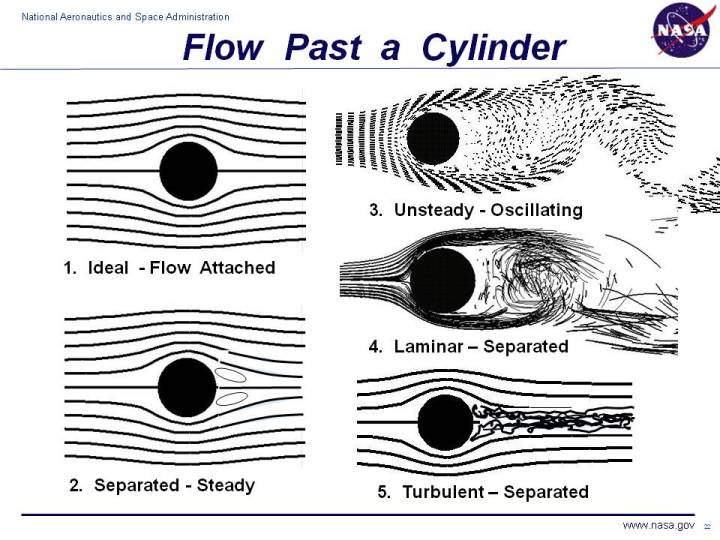
\includegraphics[scale=0.4]{flow_around_cylinders}
        \caption{Various types of flow around a cylinder extending into the page}
        \label{fig:flow types}
    \end{figure}

    Figure~\ref{fig:flow types}\footnote{https://www.grc.nasa.gov/www/K-12/airplane/dragsphere.html} shows 5 different types of flow around a cylinder extending down into the page. These are:
    \begin{enumerate}
        \item Ideal, attached flow. \(Re<0.5\)
        \item Separated, steady flow. \(Re\in[1,10]\)
        \item Separated, unsteady flow, oscillating. \(Re\in[250,10^4]\)
        \item Laminar, separated flow. \(Re\in[10^4, \num{2e5}]\)
        \item Turbulent, separated flow. \(Re>\num{2e5}\)
    \end{enumerate}
    
    \section{Drag}
    A bluff body is one that is not streamlined. Flow past a bluff body (external flow) can be split into three regions:
    
    \begin{itemize}
        \item Main ``free stream", largely undisturbed flow - found away from the body
        \item Boundary layer flow - found adjacent to the body
        \item Separated region (wake) - found trailing behind the body where the boundary layer separates from the surface
    \end{itemize}

    There are two important points on the body:
    
    \begin{itemize}
        \item Separation point - where the boundary layer leaves the body to become the wake
        \item Stagnation point - where the fluid builds up at the front of the body
    \end{itemize}

    Drag is a general term for force on a body in a downstream direction due to a fluid. 
    Drag opposes motion of the body trying to move through the fluid. Flow past a bluff body results in form drag. 
    The physical mechanism for form drag is:
    
    \begin{itemize}
        \item Re-circulation in the wake
        \item Energy loss in the wake due to viscous friction
        \item Energy loss leads to pressure decrease in the wake
        \item Flowing of fluid in front of the stagnation point increases the pressure
        \item Pressure difference is felt as a force
    \end{itemize}

    The form drag equation is
    \[F_D=\frac{1}{2}C_D\rho Au^2\]
    where \(F_D\) is the form drag force, \(C_D\) is the coefficient of drag for the shape of the body, 
    \(A\) is the projected frontal area, \(\rho\) and \(u\) are density and flow speed as usual.
    
    Some common drag coefficients are given in table~\ref{tab:common drag coefficients}
    \begin{table}[ht]
        \centering
        \begin{tabular}{c|c}
            Object & \(C_D\) \\ \hline
            Older car/truck & 0.6 to 0.8\\
            Modern car & \(\sim 0.25\)\\
            Racing car & \(\sim 0.18\)\\
            Cylinder & \(\sim 1\)
        \end{tabular}
        \caption{Common drag coefficients \(C_D\)}
        \label{tab:common drag coefficients}
    \end{table}

    Vertex shedding is the process shown in Figure~\ref{fig:flow types} in the third case. 
    Vortices build up either side of the object and come off one at a time. 
    This causes a transverse lift force perpendicular to the drag force. 
    This can cause a problem if the frequency of the vortex shedding is near that of the object.
    The frequency of vortex shedding \(f\) around an object diameter \(D\) in fluid speed \(u\) satisfies:
    \[\frac{fD}{u}=0.198\left(1-\frac{19.7}{Re}\right)\]
    For \(Re\in[250, \num{2e5}]\). 
    \(fD/u\) is the Strouhal number. 
    For a cylinder this comes out as approximately 0.2. 

    \section{Different Flows}
    
    The boundary layer thickness \(\delta\) is the distance from the wall at which \(u=0.99 u_\infty\) where \(u_\infty\) is the undisturbed flow speed.
    As you move down the surface in the direction of the flow the boundary layer thickness increases.
    The boundary layer can be laminar or turbulent.
    We can use Reynold's numbers to suggest the flow type.
    In this case the Reynold's number \(Re_x\) at distance \(x\) from the start of the surface is calculated as
    \[Re_x = \frac{\rho u_\infty x}{\mu}\]
    The laminar to turbulent transition is approximately the range \([10^5, \num{2e5}]\).
    We use different models to calculate \(\delta\) depending on the flow type:
    \[
        \begin{array}{cccc}
            \text{Laminar:} & \delta = \frac{5x}{Re_x^{1/2}}, & \delta \propto x^{1/2}, & \delta \propto u_\infty^{-1/2}\\[0.5cm]
            \text{Turbulent:} & \delta = \frac{0.37x}{Re_x^{1/5}}, & \delta \propto x^{4/5}, & \delta \propto u_\infty^{-1/5}
        \end{array}
    \]
    Since the liquid is slowed by the plate Newton's third law means that an equivalent shear force must be exerted on the surface in the direction of flow.
    This force is the skin friction drag \(F\):
    \[F=\frac{1}{2}C_f\rho Au_\infty^2\]
    where \(A\) is the wetted surface area (area in contact with the liquid) and \(C_f\) if the skin friction drag coefficient. 
    The value of \(C_f\) depends on the flow type:
    \[
        \begin{array}{cc}
            \text{Laminar:} & C_f = \frac{1.4}{Re_x^{1/2}}\\[0.5cm]
            \text{Turbulent:} & C_f = \frac{0.074}{Re_x^{1/5}}
        \end{array}
    \]
    
    \subsection{Orifice Flow}
    \begin{figure}[ht]
        \centering
        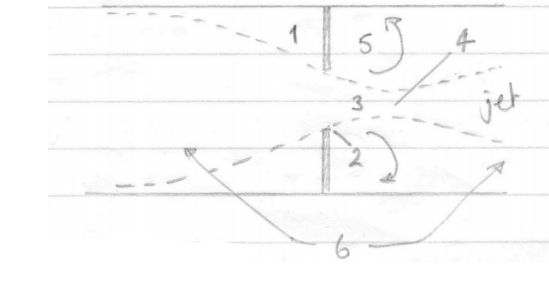
\includegraphics{orifice_flow.png}
        \caption{Flow at an orifice}
        \label{fig:orifice flow}
    \end{figure}
    Figure \ref{fig:orifice flow} shows flow at a narrowing and then widening of a pipe. 
    The areas of interest are:
    \begin{enumerate}
        \item Stagnant region
        \item Separation at the lip of the orifice
        \item Inward flow just after the orifice due to the inward inertia of the liquid
        \item The vena contracta (narrowest point) in the jet. The cross sectional area of the vena contracta is less than that of the orifice
        \item Recirculation outside of the jet
        \item Pressure drop across the orifice and therefore an energy loss
    \end{enumerate}

    \subsection{Flow Around a Sharp Bend}
    \begin{figure}[ht]
        \centering
        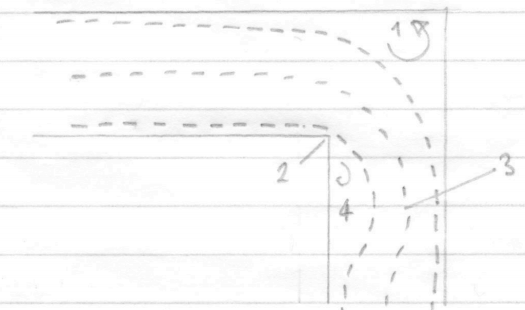
\includegraphics{sharp_bend_flow.png}
        \caption{Flow around a sharp bend}
        \label{fig:sharp bend flow}
    \end{figure}
    Figure \ref{fig:sharp bend flow} shows flow around a sharp bend.
    The areas of interest are:
    \begin{enumerate}
        \item Separation and recirculation at the outside corner
        \item Separation at the inside corner
        \item Vena contracta just downstream of the corner. This means there is a pressure drop afterwards so there is a loss of energy
        \item Recirculation
    \end{enumerate}

    \section{Dimensional Analysis}
    \example
    Estimate the skin friction drag on the body of an A380 shortly after take off.
    \[F = \frac{1}{2}C_f\rho Au^2\]
    Shortly after take off so we can use sea level properties of air which are given on the data sheet.
    Specifically \(\rho_{\text{air}} = \SI{1.2}{kg.m^{-3}}\) and \(\mu = \SI{1.8e-5}{kg.m^{-1}.s^{-1}}\).
    
    \(A\) is the area in contact with the fluid. 
    We can model the plane as a cylinder height \(L = \SI{70}{m}\) and diameter \(D = \SI{7.8}{m}\). 
    Note that there is no skin friction on either end of the cylinder as these areas have no fluid passing them and instead experience form drag.
    \[A = \pi DL \approx 3.14\cdot 7.8\cdot 70\approx \SI{1700}{m^2}\]
    We can calculate the Reynold's number of the flow, we use \(x = L\) as this gives us the maximum value for the Reynold's number.
    \(u\approx\SI{100}{m.s^{-1}}\).
    \[Re_x = \frac{\rho ux}{\mu} \approx \frac{1.2\cdot 100\cdot 70}{\num{1.8e-5}}\approx \num{470e6}\]
    \(Re_x > \num{2e5}\) so it is turbulent flow. This means we need the turbulent model for \(C_f\)
    \[C_f = \frac{0.074}{Re_x^{1/5}} \approx \frac{0.074}{\left(\num{470e6}\right)^{1/5}} \approx \num{1.36e-3}\]
    \[F = \frac{1}{2}C_f\rho Au^2 \approx \frac{1}{2}\cdot \num{1.36e-3}\cdot 1.2\cdot 1700\cdot 100^2\approx \SI{14000}{N}\]
    
    \subsection{Dimensional Analysis}
    Dimensions either side of the \(=\) sign must be the same. Three common base dimensions in mechanics are mass, \(M\), length, \(L\) and time, \(T\).
    
    \example
    Experiments suggest that \(F_D = f(u, D, \rho)\). 
    From this we hypothesise that \(F_D = Cu^aD^b\rho^c\) for some constants \(a\), \(b\), \(c\) and \(C\). 
    We can calculate values for \(a\), \(b\) and \(c\) by doing dimensional analysis:
    \begin{align*}
        [F_D] &= [u^aD^b\rho^c]\\
        &= [u^a][D^b][\rho^c]\\
        &= [u]^a[D]^b[\rho]^c\\
        [F_D] &= MLT^{-2}\\
        [u] &= LS^{-1}\\
        [D] &= L\\
        [\rho] &= ML^{-3}\\
        MLT^{-2} &= (LT^{-1})^a(L)^b(ML^{-3})^c\\
        &= L^aT^{-a}L^bM^cL^{-3c}\\
        &= M^CL^{a+b-3c}T^{-a}\\
        c &= 1\\
        a &= 2\\
        1 &= a + b - 3c\\
        b &= 2\\
        F_D &\propto \rho D^2u^2\\
        F_D &\propto \rho Au^2
    \end{align*}
    
    Further experiments determine that \(C\) isn't actually constant outside of the range of the previous experiment.
    We hypothesise that \(F_D = f(u, D, \rho, \mu)\)
    \begin{align*}
        [F_D] &= [u]^a[D]^b[\rho]^c[\mu]^d\\
        [\mu] &= ML^{-1}T^{-1}\\
        MLT^{-2} &= L^aT^{-a}L^bM^cL^{-3c}M^dL^{-d}T^{-d}\\
        MLT^{-2} &= M^{c + d}L^{a + b - 3c - d}T^{-a-d}\\
        1 &= c + d\\
        1 &= a + b - 3c - d\\
        2 &= a + d\\
        \intertext{We only have three equations and four unknowns so the best we can do is reduce the system to one unknown}
        c &= 1 - d\\
        a &= 2 - d\\
        1 &= (2 - d) + b - 3(1 - d)\\
        b &= 2 - d\\
        F_D &= g(u^{2-d}, D^{2-d}, \rho^{1-d}, \mu^d)\\
        \intertext{Where \(g\) combines its arguments linearly}
        F_D &\propto u^{2-d}D^{2-d}\rho^{1-d}\mu^d\\
        F_D &\propto \left(\frac{\rho u D}{\mu}\right)^{-d}\rho D^2u^2\\
        F_D &\propto \left(\frac{\rho u D}{\mu}\right)^{-d}\rho Au^2\\
        F_D &\propto Re^{-d}\rho Au^2
    \end{align*}
    
    \subsection{Pressure}
    A static fluid is one where there are no shearing forces. This means that all forces at a boundary must be normal to the boundary.
    
    Pressure is the force per unit area. We consider the force \(\delta F\) as we shrink the area \(\delta A\) to 0.
    \[p = \frac{\delta F}{\delta A}\]
    \[\lim_{\delta A\to 0} \frac{\delta F}{\delta A} = \dv{F}{A}\]
    The units of pressure are \(\si{N.m^{-2}} = \si{Pa}\) (pascals).
    
    Standard atmospheric pressure at sea level is \SI{101}{kPa} (strictly \SI{101.325}{kPa}).
    
    Another unit of pressure is the \si{bar} where \(\SI{1}{bar} = \SI{100}{kPa}\) \((\SI{1}{mbar} = \SI{100}{Pa})\).
    
    Pressure above absolute vacuum is known as the absolute pressure. It is measured using a barometer.
    Gauge pressure is the absolute pressure \(-\) the atmospheric pressure.
    \begin{figure}[ht]
        \centering
        \begin{tikzpicture}[yscale=0.7]
            %\draw[lightgray] (-3, 0) grid (6, 4);
            \draw (0, 0) -- (2, 0) node[right] at (2, 0) {\(p = 0\)};
            \draw (0, 4) -- (2, 4) node[right] at (2, 4) {Absolute Pressure};
            \draw[dashed] (0, 3) -- (2, 3) node[right] at (2, 3) {Gauge Pressure};
            \draw[->] (0.5, 0) -- (0.5, 4);
            \draw[->] (1, 0) -- (1, 3);
            \draw[->] (1.5, 3) -- (1.5, 4);
            \draw (-3, 0) circle (0cm);  % 0 radius circle off to right to force it to center on the diagram rather than the labels on the right
        \end{tikzpicture}
        \caption{The lengths of the arrows are (from left to right): Absolute Pressure, Atmospheric Pressure and Gauge Pressure}
    \end{figure}
    
    \section{Manometers}
    \begin{figure}[ht]
        \centering
        \begin{tikzpicture}
            %\draw[lightgray] (0, 0) grid (3, 3);
            \draw (1, 1) -- (2, 1) -- (2, 2) -- (1, 2) -- (1, 1);
            \draw[->] (0, 1) -- (0, 2) node[above] at (0, 2) {\(z\)};
            \draw[->] (1.5, 3) -- (1.5, 2) node[above] at (1.5, 3) {\(p_2\)};
            \draw[->] (1.5, 0) -- (1.5, 1) node[below] at (1.5, 0) {\(p_1\)};
            \draw[dashed] (2, 2) -- (2.5, 2) node[right] at (2.5, 2) {\(z_2\)};
            \draw[dashed] (2, 1) -- (2.5, 1) node[right] at (2.5, 1) {\(z_1\)};
        \end{tikzpicture}
        \caption{Vertical pressures on a fluid element}
        \label{fig:vertical pressure}
    \end{figure}
    Consider the fluid element in figure \ref{fig:vertical pressure}.
    It has cross sectional area \(A\) parallel to the \(x\), \(y\) plane.
    The fluid is static therefore all forces on it must cancel.
    \begin{itemize}
        \item The force on the fluid due to \(p_1\) is \(p_1A\) upwards
        \item The force on the fluid due to \(p_2\) is \(p_2A\) downwards
        \item The force on the fluid due to gravity is \(\rho gA(z_2-z_1)\) downwards
    \end{itemize}
    \[p_1A - p_2A - \rho gA(z_2 - z_1) = 0\]
    \[p2 - p1 = -\rho g(z_2 - z_1)\]
    \[\Delta p = -\rho g\Delta z\]
    \[\frac{\Delta p}{\Delta z} = -\rho g\]
    \[\lim_{\Delta z\to 0}\frac{\Delta p}{\Delta z} = \lim_{\Delta z\to 0}-\rho g = -\rho g = \dv{p}{z}\]
    If instead there are two fluids as in figure \ref{fig:two fluids pressure} then the same logic dictates that
    \[p_2 - p_1 = -\rho_yg(z_2 - z_i) - \rho_xg(z_i - z_1)\]
    \begin{figure}[ht]
        \centering
        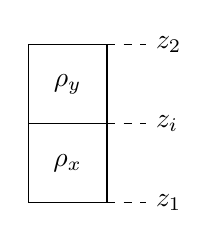
\begin{tikzpicture}
            \draw (0, 0) -- (1, 0) -- (1, 2) -- (0, 2) -- (0, 0);
            \draw (0, 1) -- (1, 1);
            \draw[dashed] (1, 0) -- (1.5, 0) node[right] at (1.5, 0) {\(z_1\)};
            \draw[dashed] (1, 1) -- (1.5, 1) node[right] at (1.5, 1) {\(z_i\)};
            \draw[dashed] (1, 2) -- (1.5, 2) node[right] at (1.5, 2) {\(z_2\)};
            \node at (0.5, 0.5) {\(\rho_x\)};
            \node at (0.5, 1.5) {\(\rho_y\)};
        \end{tikzpicture}
        \caption{Pressure in two fluids}
        \label{fig:two fluids pressure}
    \end{figure}
    We can also consider the horizontal forces acting on the fluid element as in figure \ref{fig:horizontal pressure} to show that the pressure is that same on all sides
    \[p_1A-p_2A = 0\implies p_1 = p_2\]
    \begin{figure}[ht]
        \centering
        \begin{tikzpicture}
            \draw (1, 0) -- (1, 1) -- (2, 1) -- (2, 0) -- (1, 0);
            \draw[->] (0, 0.5) -- (1, 0.5) node[left] at (0, 0.5) {\(p_1\)};
            \draw[->] (3, 0.5) -- (2, 0.5) node[right] at (3, 0.5) {\(p_2\)};
        \end{tikzpicture}
        \caption{Horizontal forces due to pressure}
        \label{fig:horizontal pressure}
    \end{figure}
    \subsection{Manometers}
    A manometer measures a pressure difference. 
    This simplest manometer is the U-tube manometer shown in figure \ref{fig:u-tube manometer}.
    In this diagram \(p_2 > p_1\).
    \[p_2-p_1 = \rho g\Delta h\]
    If \(p_1\) is atmospheric pressure then \(p_2\) is gauge pressure.
    \begin{figure}[ht]
        \centering
        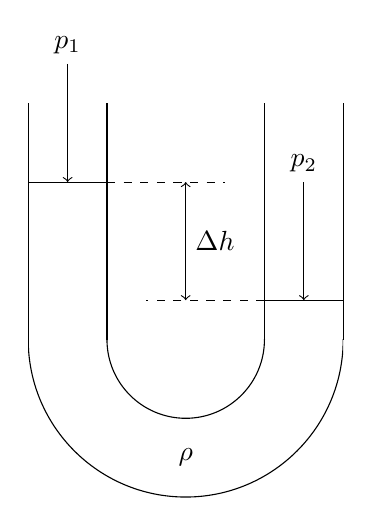
\begin{tikzpicture}
            %\draw[lightgray] (-3, 0) grid (3, 6);
            \begin{scope}
                \clip (-2, 2) rectangle (2, 0);
                \draw (0, 2) circle (2);
                \draw (0, 2) circle (1);
            \end{scope}
            \draw (-2, 2) -- (-2, 5);
            \draw (-1, 2) -- (-1, 5);
            \draw (1, 2) -- (1, 5);
            \draw (2, 2) -- (2, 5);
            \draw (-2, 4) -- (-1, 4);
            \draw (2, 2.5) -- (1, 2.5);
            \draw[->] (-1.5, 5.5) -- (-1.5, 4);
            \draw[->] (1.5, 4) -- (1.5, 2.5);
            \node[above] at (-1.5, 5.5) {\(p_1\)};
            \node[above] at (1.5, 4) {\(p_2\)};
            \draw[dashed] (-1, 4) -- (0.5, 4);
            \draw[dashed] (1, 2.5) -- (-0.5, 2.5);
            \draw[<->] (0, 4) -- (0, 2.5);
            \node[right] at (0, 3.25) {\(\Delta h\)};
            \node at (0, 0.5) {\(\rho\)};
        \end{tikzpicture}
        \caption{U-tube manometer}
        \label{fig:u-tube manometer}
    \end{figure}
    A more accurate manometer is the inclined arm manometer shown in figure \ref{fig:inclined arm manometer}. 
    This is more accurate as the length measured \(\Delta L\) is larger for the same pressure difference so the percentage error is smaller.
    Another improvement is that on one side a large reservoir has been added which means that the height on that side is only negligibly affected by changes in the height of the liquid on the other side.
    This means we only need to measure the height of the difference on one side which reduces our error.
    \[p_2 - p_1 = \rho g\Delta h = \rho g\Delta L\sin\vartheta\]
    
    \begin{figure}[ht]
        \centering
        \begin{tikzpicture}
            %\draw[lightgray] (0, 0) grid (8, 8);
            \draw (0, 7) -- (0, 5) -- (1, 5);
            \draw (2, 5) -- (3, 5) -- (3, 7);
            \draw (0, 6.5) -- (3, 6.5);
            \draw (1, 5) -- (1, 0);
            \draw (2, 5) -- (2, 2);
            \draw (2, 2) -- (7, 7);
            \draw (1, 0) -- (8, 7);
            \draw[->] (1.5, 7.5) -- (1.5, 6.5);
            \node[above] at (1.5, 7.5) {\(p_1\)};
            \draw[->] (7.5, 8) -- (7.5, 7);
            \node[above] at (7.5, 8) {\(p_2\)};
            \draw (4, 4) -- (5, 4);
            \draw[dashed] (3, 6.5) -- (7.5, 6.5);
            \draw[dashed] (4, 4) -- (3, 4);
            \draw[<->] (3.5, 4) -- (3.5, 6.5);
            \node[right] at (3.5, 5.25) {\(\Delta h\)};
            \draw[<->] (7.6, 6.4) -- (5.1, 3.9);
            \node at (6.5, 4.8) {\(\Delta L\)};
            \draw[dashed] (1, 0) -- (2, 0);
            \node at (1.5, 0.25) {\(\vartheta\)};
        \end{tikzpicture}
        \caption{Inclined arm manometer}
        \label{fig:inclined arm manometer}
    \end{figure}
    One final improvement that can be made is to use two fluids. 
    If the fluid in the manometer has density \(\rho_y\) and the other fluid has density \(\rho_x\) then the pressure difference either side of the manometer is
    \[p_2-p_1 = (\rho_y - \rho_x)g\Delta h\]
    To decrease percentage error we make \(\rho_y - \rho_x\) as big as possible. 
    For this reason we often use mercury as the liquid in the manometer as it has such a high density.
    
    \section{Pressure on Submerged Areas}
    \begin{figure}[ht]
        \centering
        \begin{tikzpicture}
            %\draw[lightgray] (0, 0) grid (15, 5);
            \draw (0, 4) -- (7, 4);
            \draw (0, 0) -- (2, 0) -- (5, 3) -- (7, 3);
            \draw[<->] (2.5, 0.5) -- (2.5, 4);
            \draw[<->] (2.6, 0.5) -- (6.1, 4);
            \node at (3.3, 0.7) {\(x\)};
            \node[above] at (6.1, 4) {\(O\)};
            \node at (5.5, 3.7) {\(\vartheta\)};
            \draw[<->] (4, 4) -- (4, 2);
            \node[right] at (4, 3) {\(\bar h\)};
            \node[right] at (2.5, 2.5) {\(h\)};
            \node at (4.2, 1.8) {\(G\)};
            
            \draw (8, 4) -- (12, 4);
            \draw (8, 0) -- (12, 0);
            \draw[fill=black] (10, 2) circle (0.05);
            \node[left] at (10, 2) {\(G\)};
            \draw[<->] (8.5, 0) -- (8.5, 4);
            \draw[<->] (11.5, 2) -- (11.5, 4);
            \node[left] at (8.5, 2) {\(h\)};
            \node[right] at (11.5, 3) {\(\bar h\)};
            \draw[dashed] (10, 2) -- (12, 2);
            \node[right] at (12, 0) {\(dA\)};
        \end{tikzpicture}
        \caption{Submerged area}
        \label{fig:submerged area}
    \end{figure}
    The submerged area shown in figure \ref{fig:submerged area} has a force acting on it due to the fluid above in.
    We can ask two questions about this force:
    \begin{enumerate}
        \item What is its magnitude?
        \item Where does it act?
    \end{enumerate}
    The fluid is static so the force must be normal to the surface.
    
    We answer these questions by considering the infinitesimal area \(dA\). 
    Since this area is so small we can approximate it at being all the same depth \(h = x\sin\vartheta\).
    The pressure \(p\) acting on \(dA\) is \(p = \rho gh\).
    The force acting on \(dA\) due to \(p\) is then
    \[dF = pdA = \rho g hdA = \rho gx\sin\vartheta dA\]
    To get the total force we integrate over all contributing \(dF\)  for elements \(dA\):
    \[\int dF = F = \int_A\rho gx\sin\vartheta\,dA = \rho g\sin\vartheta\int_A x\,dA\]
    The centroid or centre of area of the wetted area is defined by \(OG = \bar x\) where \(\int_A x\,dA = A\bar x\).
    This allows us to rewrite the force as
    \[F = \rho g\bar x A\sin\vartheta = \rho g A\bar h\]
    So the force is the pressure at the centroid times the total wetted area.
    
    The point where the force acts is known as the centre of pressure or the centre of force.
    We can consider elements \(\delta F_i\) of the force which act at a depth of \(h_i = x_i\sin\vartheta\).
    We call the total force \(F_\text{tot}\) and it acts at a depth \(x_F\).
    We consider the total affect of all elements as the size decreases and the number of elements increases.
    \[x_F F_\text{tot} = \sum_{i = 1}^{n}x_i\delta F\]
    \[\lim_{n\to\infty}\sum_{i = 1}^{n}x_i\delta F = \int x\,dF\]
    The moment \(dM\) about \(O\) due to the force \(dF\) acting on area \(dA\) is
    \[dM = xdF = x\rho g h dA = x\rho g x\sin\vartheta dA = \rho gx^2\sin\vartheta dA\]
    We integrate over all contributions \(dF\) to get
    \[\int dM = M = \int x\,dF = x_F F_\text{tot} = \int_A \rho g\sin\vartheta x^2\,dA = \rho g\sin\vartheta\int_A x^2\,dA\]
    From this we can work out the distance \(x_F\)
    \begin{align*}
        x_F &=\frac{M}{F_\text{tot}}\\
        &= \frac{\rho g\sin\vartheta\int_Ax^2\,dA}{\rho g\sin\vartheta\int_Ax\,dA}\\
        &= \frac{\int_A x^2\,dA}{\int_A x\,dA}\\
        &= \frac{1}{A\bar x}\int_A x^2\,dA
    \end{align*}
    For some common shapes we are given the value of \(x_F\).
    For a rectangle height \(d\) with its centroid at depth \(\bar x\)
    \[x_F = \frac{d^2}{12\bar x} + \bar x\]
    For a circle diameter \(d\) with its centroid at depth \(\bar x\)
    \[x_F = \frac{d^2}{16\bar x} + \bar x\]
    
    \section{Fluid Dynamics}
    Fluid motion is usually very complex.
    Motion of a fluid particle is determined by:
    \begin{itemize}
        \item Their inertia (inertial forces)
        \item Shear stresses due to surrounding fluid (viscous forces)
        \item Forces due to gradients in pressure
    \end{itemize}
    For a fluid particle \(\text{inertial force}:\text{viscous force} \propto Re\)
    
    \subsection{Definitions}
    \begin{itemize}
        \item Pathline - The line travelled by a fluid element as time passes.
        \item Streakline - The line joining the positions of all elements which have passed through a certain point. 
        This is the line created by dye injected into the flow.
        In a steady flow a pathline and streakline are the same
        \item Streamline - A line across which there is no flow.
        Local velocity is tangential to a streamline.
        \item Streamtube - A bundle of adjacent streamlines.
        Because there is no flow across a streamline a streamtube is like an imaginary pipe.
        \item Steady flow - flow where the velocity at any point doesn't change with time
        \item One dimensional flow - flow in one direction.
        Cross stream variations average out.
        Lots of flows can be approximated as 1D plus a correction factor.
        \item Uniform flow - flow where at any given instant all points have the same velocity
    \end{itemize}
    
    \subsection{Continuity Equation}
    We apply the principal of conservation of mass to a 1D steady flow.
    The volume flowrate (aka discharge) \(Q\) (aka \(q\) or \(\dot V\)) is the volume of fluid passing through a given cross section per unit time.
    \([Q] = \si{m^3.s^{-1}} = \text{cumecs}\).
    
    \begin{figure}[ht]
        \centering
        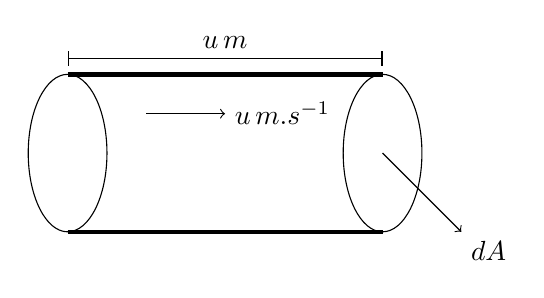
\begin{tikzpicture}
            %\draw[lightgray] (0, 0) grid (4, 2);
            \draw[ultra thick] (0, 0) -- (4, 0);
            \draw[ultra thick] (0, 2) -- (4, 2);
            \begin{scope}[yscale=2, yshift=-0.5cm]
                \draw (0, 1) circle (0.5);
                \draw (4, 1) circle (0.5);
            \end{scope}
            \draw[->] (1, 1.5) -- (2, 1.5) node[right] at (2, 1.5) {\(u\,\si{m.s^{-1}}\)};
            \draw[->] (4, 1) -- (5, 0) node[below right] at (5, 0) {\(dA\)};
            \draw[|-|] (0, 2.2) -- (4, 2.2) node[above] at (2, 2.2) {\(u\,\si{m}\)};
        \end{tikzpicture}
        \caption{Volume flow rate through area \(dA\)}
        \label{fig:volume flow rate through area dA}
    \end{figure}
    For the fluid shown in figure \ref{fig:volume flow rate through area dA} since the fluid is moving at \(u\,\si{m.s^{-1}}\) all fluid within a distance of \(u\,\si{m}\) of the area \(dA\) will flow through \(dA\).
    
    The mass flowrate \(\dot m\) is the mass of fluid passing through a given cross section per unit time.
    \([\dot m]=\si{kg.s^{-1}}\).
    \[m = \rho V\implies \dot m = \rho\dot V = \rho Q\]
    \[\implies d\dot m = \rho dQ = \rho u dA\]
    \[\implies \int d\dot m = \int_A \rho\,dQ = \int_A \rho u\,dA\]
    
    \subsection{Ideal Flow}
    Ideal flow is inviscid (no viscosity, free slip and uniform) and incompressible.
    This means that \(u\) is constant across the duct.
    The fluid has a flat velocity profile \(u(y) = u\)
    \[\dot m = \int_A \rho u\,dA =\rho u\int dA = \rho uA\]
    For two cross sections 1 and 2:
    \[\dot m = \rho u_1A_1 = \rho u_2A_2\]
    in an ideal fluid \(\rho\) is constant so
    \[u_1A_1 = u_2A_2 = Q\]
    
    \subsection{Non-Ideal Flow}
    In non-ideal flow \(u\) varies across the duct.
    The mean velocity \(\bar u\) can be calculated using the volume flowrate
    \[\bar u = \frac{Q}{A}\]
    \[\dot m = \rho \bar u_1A_1 = \rho \bar u_2A_2\]
    
    \example
    A rectangular duct shown in figure \ref{fig:flow in rectangular duct} has dimensions \(b\times 2a\)
    \begin{figure}[ht]
        \centering
        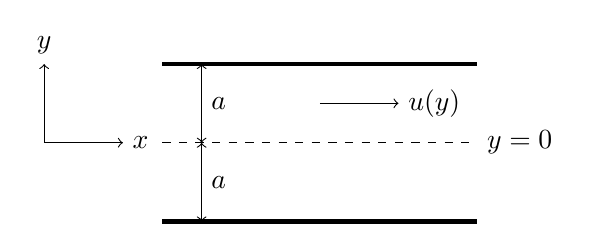
\begin{tikzpicture}
            \draw[ultra thick] (0, 0) -- (4, 0);
            \draw[ultra thick] (0, 2) -- (4, 2);
            \draw[dashed] (0, 1) -- (4, 1) node[right] at (4, 1) {\(y=0\)};
            \draw[<->] (-1.5, 2) -- (-1.5, 1) -- (-0.5, 1);
            \node[above] at (-1.5, 2) {\(y\)};
            \node[right] at (-0.5, 1) {\(x\)};
            \draw[<->] (0.5, 0) -- (0.5, 1);
            \draw[<->] (0.5, 1) -- (0.5, 2);
            \node[right] at (0.5, 0.5) {\(a\)};
            \node[right] at (0.5, 1.5) {\(a\)};
            \draw[->] (2, 1.5) -- (3, 1.5) node[right] at (3, 1.5) {\(u(y)\)};
        \end{tikzpicture}
        \caption{Flow in a rectangular duct}
        \label{fig:flow in rectangular duct}
    \end{figure}

    \[\dot m = \rho \int_A u(y)\,dA\]
    \[dA = bdy\]
    \[\dot m = \rho \int_A u(y) b\,dy = \rho b\int_A u(y)\,dy = \rho b\int_{-a}^a u(y)\,dy\]
    For laminar flow we have
    \[u(y) = u_\text{max}\left(1 - \frac{y^2}{a^2}\right)\]
    A quick sanity check shows that this is 0 at \(y = a\) as we are at a boundary and the no slip condition applies and at a maximum \(y = 0\) which is what we would expect.
    \begin{align*}
        \dot m &= \rho b\int_{-a}^a u_\text{max} - \frac{y^2}{a^2} u_\text{max}\,dy\\
        &= \rho bu_\text{max}\left[y - \frac{y^3}{3a^2}\right]_{-a}^a\\
        &= \rho bu_\text{max}\left(a - \frac{a^3}{3a^2} + a - \frac{a^3}{3a^2}\right)\\
        &= \rho bu_\text{max}\frac{4a}{3}\\
        &= \frac{4}{3}\rho abu_\text{max}
    \end{align*}
    \[\implies \bar u = \frac{Q}{A} = \frac{\dot m}{\rho}\frac{1}{2ab}=\frac{2}{3}u_\text{max}\]
    
    \example
    A circular pipe as shown in figure \ref{fig:flow in circular pipe} has radius \(R\).
    \begin{figure}[ht]
        \centering
        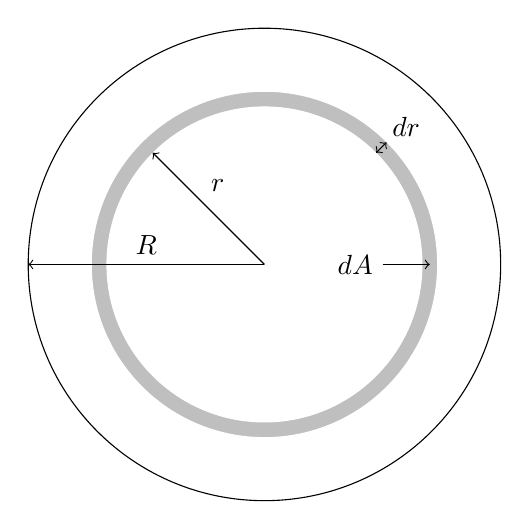
\begin{tikzpicture}
            \draw (0, 0) circle (3);
            \draw[color=white, fill=lightgray] (0, 0) circle (2.2);
            \draw[color=white, fill=white] (0, 0) circle (2);
            \draw[->] (0, 0) -- (-1.418, 1.418);
            \node[above right] at (-0.8, 0.8) {\(r\)};
            \draw[->] (0, 0) -- (-3, 0);
            \node[above] at (-1.5, 0) {\(R\)};
            \draw[<->] (1.418, 1.418) -- (1.55, 1.55);
            \node[above right] at (1.5, 1.5) {\(dr\)};
            \draw[->] (1.5, 0) -- (2.1, 0) node[left] at (1.5, 0) {\(dA\)};
            
            %\draw[lightgray] (-3, -3) grid (3, 3);
        \end{tikzpicture}
        \caption{Flow in a circular pipe}
        \label{fig:flow in circular pipe}
    \end{figure}
    \[dA = 2\pi rdr\]
    \[\dot m = \rho \int_A u(r)\,dA = \rho \int_0^R u(r)\cdot2\pi r\,dr = 2\pi\rho\int_0^R u(r)r\,dr\]
    For laminar flow we have
    \[u(r) = u_\text{max}\left(1 - \frac{r^2}{R^2}\right)\]
    As a quick sanity check this is 0 when \(r = R\) which is next to a boundary so the no slip condition applies and it is a maximum at \(r = 0\) as we would expect.
    \begin{align*}
        \dot m &= 2\pi\rho u_\text{max}\int_0^R r - \frac{r^3}{R^2}\,dr\\
        &= 2\pi\rho u_\text{max}\left[\frac{r^2}{2} - \frac{r^4}{4R^2}\right]_0^R\\
        &= 2\pi\rho u_\text{max}\left(\frac{R^2}{2} - \frac{R^4}{4R^2}\right)\\
        &= 2\pi\rho u_\text{max}\left(\frac{R^2}{2} - \frac{R^2}{4}\right)\\
        &= \pi\rho u_\text{max}\frac{R^2}{2}\\
    \end{align*}
    \[\bar u = \frac{Q}{A} = \frac{\dot m}{\rho}\frac{1}{\pi R^2} = \frac{1}{2} u_\text{max}\]
    
    \subsection{Equation of Motion}
    We want to derive the equation of motion along a streamline for an ideal fluid.
    If instead of an ideal fluid we considered viscous force then we would get the Navier-Stokes equations.
    We define the \(\vh s\) direction as along a streamline.
    Note that \(\dot{\vh s}\ne \vv 0\) in general as the direction of flow change with time.
    By definition of a streamline all velocity local to it is in the \(\vh s\) direction, that is \(\vv u = u\vh s\).
    We consider the fluid element shown in figure \ref{fig:fluid element for eqn of motion}
    
    \begin{figure}[ht]
        \centering
        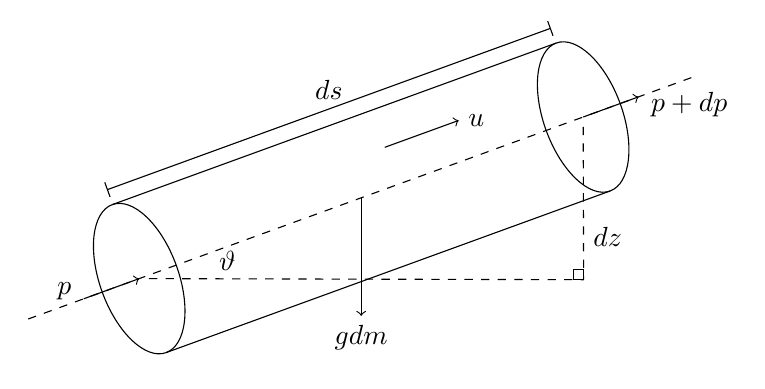
\begin{tikzpicture}
            %\draw[lightgray] (-1, -1) grid (7, 5);
            \begin{scope}[rotate around={20:(3, 1)}]
                \draw (0, 0) -- (6, 0);
                \draw (0, 2) -- (6, 2);
                \begin{scope}[yscale=2]
                    \draw (0, 0.5) circle (0.5);
                    \draw (6, 0.5) circle (0.5);
                \end{scope}
                \draw[dashed] (-1.5, 1) -- (7.5, 1);
                \draw[->] (3.5, 1.5) -- (4.5, 1.5) node[right] at (4.5, 1.5) {\(u\)};
                \draw[|-|] (0, 2.2) -- (6, 2.2) node[above] at (3, 2.2) {\(ds\)};
                \draw[->] (-0.75, 1) -- (0, 1) node[left] at (-0.75, 1.1) {\(p\)};
                \draw[->] (6, 1) -- (6.75, 1) node[right] at (6.75, 0.9) {\(p + dp\)};
                \node (left area) at (0, 1) {};
                \node (right area) at (6, 1) {};
            \end{scope}
            \draw[->] (3, 1) -- (3, -0.5) node[below] at (3, -0.5) {\(gdm\)};
            \draw[dashed] (left area) -- (5.825, -0.04);
            \draw[dashed] (right area) -- (5.825, -0.04);
            \draw (5.7, -0.04) rectangle (5.825, 0.085);
            \node[right] at (5.825, 0.5) {\(dz\)};
            \node at (1.3, 0.2) {\(\vartheta\)};
        \end{tikzpicture}
        \caption{Fluid element for the derivation of the equation of motion}
        \label{fig:fluid element for eqn of motion}
    \end{figure}
    
    We consider each force individually and then combine them to apply Newton's second law.
    It is also useful to consider the force per unit volume instead of force which leaves us with mass per unit volume \(= \rho\).
    \subsubsection*{Force Due to Gravity}
    \[F_g = -gdm\sin\vartheta\]
    Sanity check:
    \[\vartheta = 0\implies F_g = 0\]
    as \(F_g\) is perpendicular to \(\vh s\) and
    \[\vartheta = \frac{\pi}{2}\implies F_g = -gdm\]
    as \(F_g\) is parallel to \(\vh s\).
    We can use basic trig to show \(\sin\vartheta = dz/ds\)
    \[F_g = -gdm\sin\vartheta = -gdm\dv{z}{s}\]
    Force due to gravity per unit volume
    \[f_g = -\rho g\dv{z}{s}\]
    
    \subsubsection*{Force Due to Pressure}
    \[F_p = p dA - (p + dp)dA = -dpdA\]
    The volume of the fluid element is given by
    \[dV = dAds\]
    Force due to pressure per unit volume
    \[f_p = dp\dv{A}{V} = -\dv{p}{s}\]
    
    \subsubsection*{Apply Newton's Second Law}
    \[F_\text{tot} = F_g + F_p = ma\]
    Calculate everything per unit volume
    \[f_\text{tot} = f_g + f_p = \frac{m}{dV}a = \rho a = \rho\dv{u}{t}\]
    \[-\dv{p}{s} - \rho g\dv{z}{s} = \rho\dv{u}{t}\]
    
    \section{Bernoulli Equation}
    \(u\) is a function of time \(t\) and position along the streamline \(s\).
    \[u = u(s, t)\]
    If we consider a small change \(\delta u\) we can write this as a combination of the contributions \(\delta s\) and \(\delta t\) due to the \(s\) and \(t\) components.
    \[\delta u = \pdv{u}{t}\delta t + \pdv{u}{s}\delta s\]
    \[\frac{\delta u}{\delta t} = \pdv{u}{t} + \pdv{u}{s}\frac{\delta s}{\delta t}\]
    \[\lim_{\delta t\to 0}\frac{\delta u}{\delta t} = \dv{u}{t} = \pdv{u}{t} + \pdv{u}{s}\pdv{s}{t} = \pdv{u}{t} + u\pdv{u}{s}\]
    This is the equation of motion for a incompressible, inviscid flow.
    The three parts of this are:
    \begin{itemize}
        \item The total (aka material or Lagrangian) acceleration:
        \[\dv{u}{t}\]
        \item The local (aka Eulerian) acceleration
        \[\pdv{u}{t}\]
        \item The convective acceleration
        \[u\pdv{u}{s}\]
    \end{itemize}
    
    \subsection{Bernoulli Equation Derivation}
    \begin{equation}\label{eqn:start eqn for bernoulli}
        \pdv{u}{t} + u\pdv{u}{s} + \frac{1}{\rho}\pdv{\rho}{s} + g\pdv{z}{s}
    \end{equation}
    Using the quotient rule:
    \[\pdv{s}\left(\frac{p}{\rho}\right) = \frac{1}{\rho}\pdv{p}{s} + \left(\frac{p}{\rho^2}\right)\pdv{\rho}{s}\]
    The first term of this appears in equation \ref{eqn:start eqn for bernoulli}.
    \[u\pdv{u}{s} = \frac{1}{2}\pdv{s}(u^2)\]
    This also appears in \ref{eqn:start eqn for bernoulli}. 
    Making both of these substitutions gives
    \[\pdv{u}{t} + \frac{1}{2}\pdv{s}(u^2) + \pdv{s}\left(\frac{p}{\rho}\right) + g\pdv{z}{s} + \left(\frac{p}{\rho^2}\right)\pdv{\rho}{s} = 0\]
    The last term in this is 0 for a incompressible flow as the density doesn't change, this is the compressible term.
    It can be ignored for incompressible flows.
    We can integrate from position 1 to position 2 which gives
    \[\int_1^2 \pdv{u}{t}\,ds + \left[\frac{u^2}{2} + \frac{p}{\rho} + gz\right]_1^2\]
    If we assume a steady flow then \(u\) is constant so
    \[\pdv{u}{t} = 0\implies \int_1^2\pdv{u}{t}\,ds = 0\]
    Substituting our limits gives
    \begin{equation}\label{eqn:bernoulli}
        \frac{u_1^2}{2} + \frac{p_1}{\rho} + gz_1 = \frac{u_2^2}{2} + \frac{p_2}{\rho} + gz_2
    \end{equation}
    This is the Bernoulli equation for steady flow.
    Each term has dimensions of energy per unit mass:
    \begin{itemize}
        \item \(u^2/2\) is kinetic energy per unit mass
        \item \(gz\) is gravitational potential energy per unit mass
        \item \(p/\rho\) is the energy stored in pressure per unit mass
    \end{itemize}
    This is because this can also be considered as a conservation of energy statement since we are integrating a force with respect to position.
    
    \subsection{Equation of Motion Perpendicular to a Streamline}
    We define a direction \(\vh r\) as perpendicular to \(\vh s\) and outwards from the centre of a circle which approximates the radius of curvature at that point.
    \begin{figure}[ht]
        \centering
        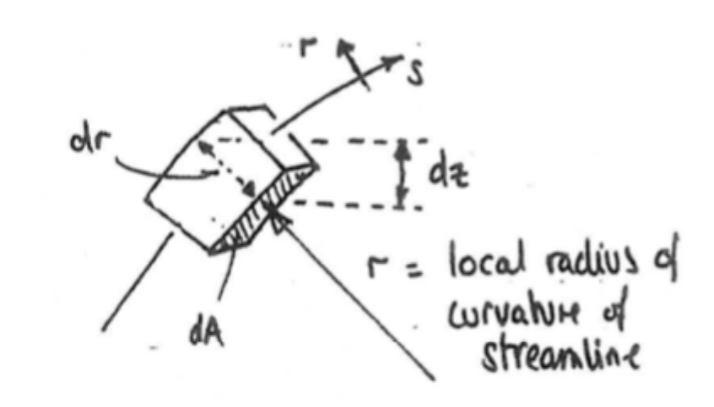
\includegraphics[scale=0.6]{perpendicular_to_streamline_1.png}
        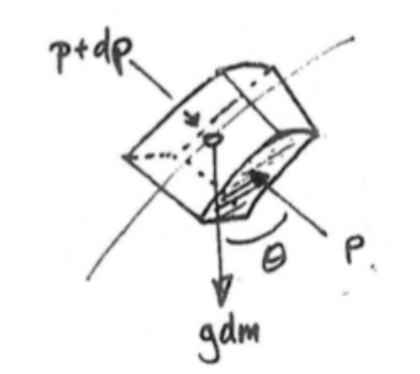
\includegraphics[scale=0.7]{perpendicular_to_streamline_2.png}
        \caption{Motion Perpendicular to a streamline}
    \end{figure}
    We can go through the same process of considering different forces and forces per unit volume
    \subsubsection*{Force Due to Gravity}
    \[\vartheta = \dv{z}{r}\]
    \[F_g = -gdm\cos\vartheta = -gdv\dv{z}{r}\]
    \(dm = \rho dV\) so the force per unit volume is
    \[f_g = -\rho g\dv{z}{r}\]
    
    \subsubsection*{Force Due to Pressure}
    \[F_p = pdA - (p + dp)dA = -pdpdA\]
    \(dV = dAdr\) so the force per unit volume is
    \[f_p = -dp\dv{A}{V} = -\dv{p}{r}\]
    
    \subsubsection*{Apply Newton's Second Law}
    Acceleration is \(u^2/r\) as this is circular motion and since we are using force per unit volume the density is used instead of the mass
    \[-\dv{p}{r} - \rho g\dv{z}{r} = -\rho \frac{u^2}{r}\]
    \[\implies \rho \frac{u^2}{r} = \dv{r}(p + \rho g z)\]
    For a straight streamline \(r \to \infty\) so \(p + \rho gz\) is constant.
    For a straight horizontal streamline the height doesn't change so \(\rho g z = 0\) but \(p + \rho g z\) is still constant so \(p\) must be constant.
    \(p + \rho g z\) is known as the piezometric pressure and is denoted \(p^*\).
    \(p^*\) is equal on adjacent straight streamlines in a horizontal flow.
    
    \section{Applying Bernoulli}
    We set the Bernoulli equation for steady flow (equation \ref{eqn:bernoulli}) equal to a constant \(\Phi\) we get
    \[\frac{u^2}{2} + \frac{p}{\rho} + gz = \Phi\]
    Where \(\Phi\) is the total energy per unit mass.
    We can multiply this by \(\rho\) to get an equation that is in terms of pressure
    \[\frac{\rho u^2}{2} + p + \rho g z = P\]
    where \(P\) is the total pressure.
    \(\rho u^2/2\) is the dynamic pressure.
    Instead we can divide by \(g\) to get
    \[\frac{u^2}{2g} + \frac{p}{\rho g} + z = H\]
    where \(H\) is the total head.
    \(u^2/(2g)\) is the velocity head and \(p/(\rho g)\) is the pressure head.
    
    There are restrictions that apply to using any of these equations:
    \begin{enumerate}
        \item Points 1 and 2 must be connected by an unbroken streamline
        \item Density \(\rho\) must be constant
        \item No energy loss between points 1 and 2
        \item Steady flow (speed at a point constant over time)
        \item No energy sources or sinks between points 1 and 2
    \end{enumerate}
    
    Some of these restrictions are more important than others:
    \begin{enumerate}
        \item This must apply
        \item This is true for a liquid or a sufficiently slow gas (\(u\ll c\), \(u<0.3 M\))
        \item For small loses we can use a correction factor (eg orifice meter)
        \item If the time scale for change in flow speed at a point over time is much larger than the time scale for the time to flow from point 1 to point 2 then we can approximate the flow as steady
        \item This must apply
    \end{enumerate}
    
    \subsection{Siphon Example}
    \begin{figure}[ht]
        \centering
        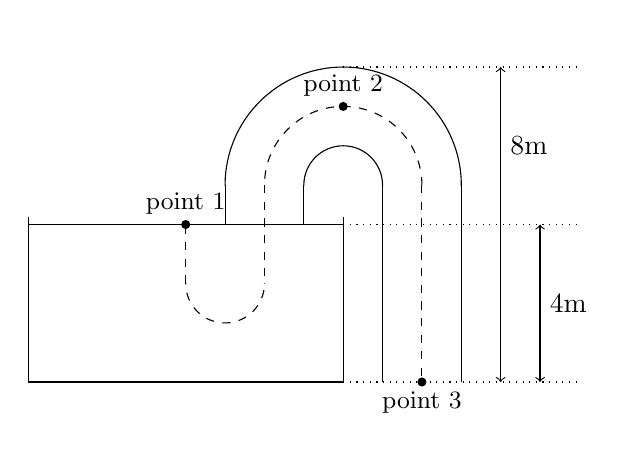
\begin{tikzpicture}
            %\draw[lightgray] (0, 0) grid (7, 5);
            \draw (0, 2.1) -- (0, 0) -- (4, 0) -- (4, 2.1);
            \draw (0, 2) -- (4, 2);
            \draw (2.5, 2) -- (2.5, 2.5);
            \draw (3.5, 2) -- (3.5, 2.5);
            \begin{scope}[yshift=-0.5cm]
                \clip (2, 5) rectangle (6, 3);
                \draw (4, 3) circle (0.5cm);
                \draw (4, 3) circle (1.5cm);
                \draw[dashed] (4, 3) circle (1cm);
            \end{scope}
            \draw (4.5, 2.5) -- (4.5, 0);
            \draw (5.5, 2.5) -- (5.5, 0);
            \draw[dashed] (5, 2.5) -- (5, 0);
            \begin{scope}
                \clip (4, 1.25) rectangle (1, 0);
                \draw[dashed] (2.5, 1.25) circle (0.5cm);
            \end{scope}
            \draw[dashed] (3, 2.5) -- (3, 1.25);
            \draw[dashed] (2, 1.25) -- (2, 2);
            \draw[dotted] (4, 4) -- (7, 4);
            \draw[dotted] (4, 0) -- (7, 0);
            \draw[dotted] (4, 2) -- (7, 2);
            \draw[<->] (6, 0) -- (6, 4);
            \draw[<->] (6.5, 0) -- (6.5, 2);
            \node[right] at (6, 3) {\SI{8}{m}};
            \node[right] at (6.5, 1) {\SI{4}{m}};
            
            \draw[fill=black] (2, 2) circle (0.05cm);
            \draw[fill=black] (4, 3.5) circle (0.05cm);
            \draw[fill=black] (5, 0) circle (0.05cm);
            \node[above] at (2, 2) {\small{point 1}};
            \node[above] at (4, 3.5) {\small{point 2}};
            \node[below] at (5, 0) {\small{point 3}};
        \end{tikzpicture}
        \caption{A siphon}
        \label{fig:siphon}
    \end{figure}
    Figure \ref{fig:siphon} shows a siphon. What is the speed \(u_3\) of the flow at point 3 given that the liquid is water and points one and three are at atmospheric pressure?
    
    Check conditions:
    \begin{enumerate}
        \item Streamline from point one to three \(\checkmark\)
        \item Liquid flow therefore density is constant \(\checkmark\)
        \item Flow is ideal enough \(\checkmark\)
        \item Flow, once established, is steady \(\checkmark\)
        \item No energy sources or sinks between points one and three \(\checkmark\)
    \end{enumerate}
    The systematic approach to solve this type of problem is:
    \begin{enumerate}
        \item Draw a diagram
        \begin{itemize}
            \item Label key points
            \item Draw a streamline joining them
        \end{itemize}
        \item Write down available information and identify what you need to find
        \item write down relevant equations
        \item Solve for the unknown
    \end{enumerate}     
    \[
        \begin{array}{cc}
            p_1 = p_\text{atm} = \SI{101}{kPa} & p_3 = p_\text{atm} = \SI{101}{kPa}\\
            z_1 = \SI{4}{m} & z_3 = \SI{0}{m}\\
            u_1 = \SI{0}{m.s^{-1}} & u_3 = \,?
        \end{array}
    \]
    We can approximate point 1 as stationary if the reservoir is large enough that changes in the height of the water are negligible, hence \(u_1=\SI{0}{m.s^{-1}}\).
    \[\frac{u_1^2}{2} + \frac{p_1}{\rho} + gz_1 = \frac{u_3^2}{2} + \frac{p_3}{\rho} + gz_3\]
    \(u_1 = 0\), \(z_3 = 0\) and \(p_1/\rho = p_3/\rho\):
    \[gz_1 = \frac{u_3}{2}\]
    \[u_3 = \sqrt{2gz_1} = \sqrt{2\cdot 4g} = \SI{8.9}{m.s^{-1}}\]
    
    What is the pressure at point 2?
    \[
        \begin{array}{cc}
            p_2 = \,? & p_3 = p_\text{atm} = \SI{101}{kPa}\\
            z_2 = \SI{8}{m} & z_3 = \SI{0}{m}\\
            u_2 = \,? & \SI{8.9}{m.s^{-1}}
        \end{array}
    \]
    \[\rho = \SI{1000}{kg.m^{-3}}\]
    We can use continuity to calculate \(u_2\). \(A_2 = A_3\) so \(A_2u_2 = A_3u_3\implies u_2 = u_3 = \SI{8.9}{m.s^{-1}}\)
    \[\frac{u_2^2}{2} + \frac{p_2}{\rho} + gz_2 = \frac{u_3^2}{2} + \frac{p_3}{\rho} + gz_3\]
    \(z_3 = 0\) and \(u_2/2 = u_3/2\):
    \[\frac{p_2}{\rho} + gz_2 = \frac{p_3}{\rho}\]
    \[p_2 = p_3 - \rho gz_2 = \SI{101}{kPa} - 8g = \SI{22.6}{kPa}\]
    This is a low value of pressure so we should consider cavitation effects
    
    \subsection{Cavitation}
    Cavitation occurs when a liquid is at a low enough pressure that gasses start to come out of solution and the liquid starts to boil. 
    This causes microscopic bubbles to form in the liquid.
    When the pressure increases again these bubbles collapse.
    If they do this against a solid surface they can cause a lot of damage over time.
    This is called cavitation erosion.
    
    \subsection{Flow Change With Area}
    If a pipe changes from cross sectional area \(A_1\) to \(A_2\) we can use Bernoulli to tell us what happens to properties of the flow as we move between these areas.
    To make things easy we consider a pipe in a horizontal plane allowing us to ignore the \(gz\) terms.
    \[p_1 + \frac{\rho u_1^2}{2} = p_2 + \frac{\rho u_2^2}{2}\]
    We can use continuity to relate \(u_1\) and \(u_2\):
    \[A_1u_1 = A_2u_2\implies u_2 = u_1\frac{A_1}{A_2}\]
    \[\implies p_2 = p_1 + \frac{\rho u_1^2}{2}\left(1 - \frac{A_1^2}{A_2^2}\right)\]
    Without loss of generality we can assume that \(A_2 < A_1\).
    This means \(A_1/A_2 > 1\).
    Hence the pressure \(p_1\) must be greater than \(p_2\) since the other term on the right hand side is negative.
    From this we can see that speed increases and pressure decreases as area decreases.
    
    \section{More Applications of Bernoulli}
    \example
    Figure \ref{fig:sharp bend flow} shows flow around a bend. 
    At point 3 indicated on the figure there is a vena contracta. 
    The bend is in a horizontal plane, the liquid is water, the flow speed before the bend is \(\SI{10}{m.s^{-1}}\) and the pressure starts as atmospheric pressure. 
    What is the pressure in the vena contracta if the area of the pipe is 1.6 times the area of the vena contracta??
    \[
        \begin{array}{cc}
            p_1 = p_\text{atm} = \SI{101}{kPa} & p_2 = \,?\\
            u_1 = \SI{10}{m.s^{-1}} & u_2 = \,?\\
        \end{array}
    \]
    \[\rho = \SI{1000}{kg.m^{-3}}\]
    \[\frac{A_1}{A_2} = 1.6\]
    We can use continuity to calculate the flow speed at the vena contracta
    \[u_1A_1 = u_2A_2 \implies u_2 = u_1\frac{A_1}{A_2}\]
    \[\frac{u_1^2\rho}{2} + p_1 = \frac{u_2^2\rho}{2} + p_2\]
    \[p_2 = \frac{u_1^2\rho}{2} + p_1 - \frac{u_2^2\rho A_1^2/A_2^2}{2} = p_2\]
    \[\frac{u_1^2\rho}{2}\left(1 - \frac{A_1^2}{A_2^2}\right) + p_1 = p_2\]
    \[\frac{10^2\,\si{m^2.s^{-2}}\cdot \SI{1000}{kg.m^3}}{2}\left(1 - \frac{A_1^2}{A_2^2}\right) + \SI{101}{kPa} = \SI{23}{kPa}\]
    This is low so we need to consider cavitation.
    
    Figure \ref{fig:orifice flow} shows flow through an orifice. 
    Point four on the diagram indicates the vena contracta of the flow.
    We assume: steady, incompressible, inviscid flow along a horizontal streamline.
    We also assume that the streamline along the middle of the pipe has no curvature.
    Find a formula for the mass flow rate.
    We take point one to be sufficiently far upstream that the flow is unaffected by the orifice and point two to be in the vena contracta.
    By Bernoulli given \(z_1 = z_2\):
    \[\frac{u_1^2}{2} + \frac{p_1}{\rho} = \frac{u_2^2}{2} + \frac{p_2}{\rho}\]
    \[u_2^2 - u_1^2 = \frac{2}{\rho}(p_1 - p_2)\]
    By continuity
    \[u_1 = u_2\frac{A_2}{A_1}\]
    \[\implies u_2^2\left(1 - \frac{A_2^2}{A_1^2}\right) = \frac{2}{\rho}(p_1 - p_2)\]
    \[u_2 = \sqrt{\frac{2(p_1 - p_2)}{\rho(1 - A_2^2/A_1^2)}}\]
    \[\dot m = \rho u_2 A_2 = \rho A_2\sqrt{\frac{2(p_1 - p_2)}{\rho(1 - A_2^2/A_1^2)}} = A_2\sqrt{\frac{2\rho(p_1 - p_2)}{1 - A_2^2/A_1^2}}\]
    There are some problems with this:
    \begin{itemize}
        \item \(A_2\) is unknown
        \item It is hard to be sure that the pressure is actually measured at the the vena contracta and not just near it
        \item Actual flow isn't ideal
    \end{itemize}
    To fix this we use an empirical correction factor.
    This takes into account the non-ideal nature of the flow as well as allowing us to use the area of the orifice \(A_o\) as opposed to the area of the vena contracta.
    The way that this is measured depends on the standard but one of the most common ones is to have point one be one pipe diameter before the orifice and point two half a pipe diameter after the orifice.
    This gives the equation
    \[\dot m_\text{actual} = CA_o\sqrt{\frac{2\rho(p_1 - p_2)}{1 - A_o^2/A_1^2}}\]
    
    \example
    A large tank has a hole at depth \(h\).
    Out of this hole liquid flows as a jet with a vena contracta. 
    Find the flow rate.
    Take point one to be on the surface of the liquid in the tank and point two to be in the vena contracta.
    Assumptions: quasi-steady flow so \(u_1 \approx 0\), there is no streamline curvature at either point, the pressure is uniform across the flow at point two, the points are connected by a streamline and the orifice is small compared to the depth.
    By Bernoulli with \(u_1 = 0\) and taking \(z_2 = 0\) which means \(z_1 = h\):
    \[\frac{p_1}{\rho} + gh = \frac{u_2^2}{2} + \frac{p_2}{\rho}\]
    \[u_2 = \sqrt{2\left(\frac{p_1 - p_2}{\rho} + gh\right)}\]
    \[Q = A_2U_2 = CA_o\sqrt{2\left(\frac{p_1 - p_2}{\rho} + gh\right)}\]
    For the special case \(p_1 = p_2 = p_\text{atm}\) we get
    \[Q = CA_o\sqrt{2gh}\]
    If instead the reservoir isn't large enough to ignore the motion of the surface then we can still use this if we make the approximation that the surface is always at some mean height \(h_m\).
    This gives
    \[u_2 = \sqrt{2gh_m}\]
    the mean flow rate is then
    \[Q_m = CA_o\sqrt{2gh_m}\]
    \[\frac{\Delta V}{\Delta t}\approx CA_o\sqrt{2gh_m}\]
    \[\Delta t \approx \frac{\Delta V}{CA_o\sqrt{2gh_m}}\]

    \section{Measuring Flow Speed}
    \begin{figure}[ht]
        \centering
        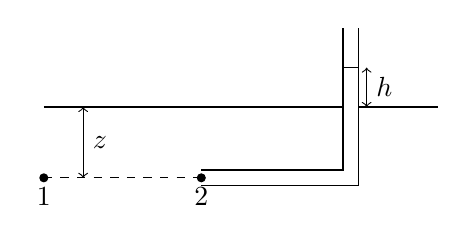
\begin{tikzpicture}
            %\draw[lightgray] (-1, 0) grid (5, 3);
            \draw (1, 1) -- (3, 1) -- (3, 3);
            \draw (1, 1.2) -- (2.8, 1.2) -- (2.8, 3);
            \draw (-1, 2) -- (2.8, 2);
            \draw (3, 2) -- (4, 2);
            \draw[dashed] (-1, 1.1) -- (1, 1.1);
            \draw[<->] (-0.5, 1.1) -- (-0.5, 2) node[right] at (-0.5, 1.55) {\(z\)};
            \draw (2.8, 2.5) -- (3, 2.5);
            \draw[<->] (3.1, 2) -- (3.1, 2.5) node[right] at (3.1, 2.25) {\(h\)};
            \draw[fill=black] (-1, 1.1) circle (0.05cm) node[below] at (-1, 1.1) {1};
            \draw[fill=black] (1, 1.1) circle (0.05cm) node[below] at (1, 1.1) {2};
        \end{tikzpicture}
        \caption{A pitot tube}
        \label{fig:pitot tube}
    \end{figure}
    Flow speed in an open channel can be measured using a pitot tube as in figure \ref{fig:pitot tube}.
    The flowing fluid forces the water level in the tube to rise by a height \(h\).
    We can assume that there is a stagnation point at 2 as there is no fluid flowing out of the tube so there can't be any flowing in.
    We also assume that point 1 is far enough upstream that it is unaffected by the tube.
    We know the velocity at 2, \(u_2 = 0\) and that \(z_1 = z_2\).
    We can use Bernoulli to get
    \[\frac{u_1^2}{2} + \frac{p_1}{\rho} = \frac{p_2}{\rho}\]
    \begin{equation}\label{eqn:pitot}
        u_1^2 = \frac{2}{\rho}(p_2 - p_1)
    \end{equation}
    The pressure at 1 is just the head pressure \(p_1 = 2\rho gz\).
    The pressure at 2 is the same as the pressure at the bend of the pitot tube since all the fluid in the tube is stationary, \(p_2 = \rho g(z + h)\).
    \[u_1 = \sqrt{2gh}\]
    
    In non-open channel flows we need to measure the pressure difference between static pressure in the duct (pressure of the undisturbed, flowing fluid) and the impact pressure at the stagnation point.
    To do this we use a pitot static tube.
    This is a pitot tube in another tube. The outer tube isn't open a the front the same as the pitot tube but rather has holes along its side, these holes allow the pressure in the outer tube to equalise to that of the fluid flowing past it.
    That is the static pressure.
    We then use the pressure difference \(\Delta p\) between the two tubes in equation \ref{eqn:pitot} to find the speed
    \[u_1 = \sqrt{\frac{2\Delta p}{\rho}}\]
    
    \subsection{Flow Over a Weir}
    \begin{figure}[ht]
        \centering
        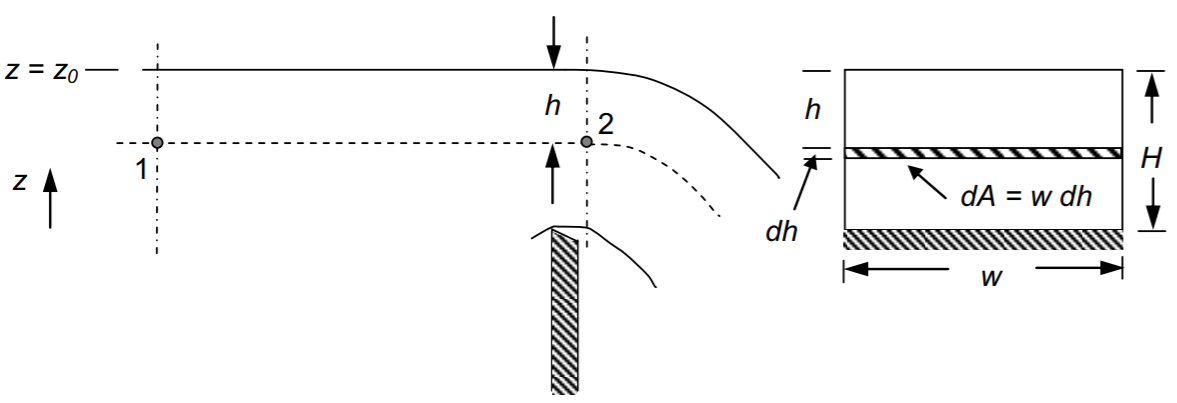
\includegraphics[scale=0.4]{flow_over_weir.png}
        \caption{Flow over a weir}
        \label{fig:flow over weir}
    \end{figure}
    Figure \ref{fig:flow over weir} shows fluid flowing over a sharp crested weir.
    There is uniform pressure in the jet in the cross section of the flow at point 2.
    This is because the jet is parallel to the surface and that is at atmospheric pressure so \(p_\text{jet} = p_\text{atm}\).
    The speed before the weir is much slower than after so \(u_1\approx 0\).
    The term \(p_1 + \rho gz_1 = p_\text{atm} + \rho gz_0 = p^*\) is constant over the cross section.
    \(p_2 = p\text{atm}\) and \(\rho g z_2 = \rho g (z_0 - h)\).
    Substituting these into the Bernoulli equation in terms of pressure gives
    \[p_\text{atm} + \rho gz_0 = \frac{\rho u_2^2}{2} + p_\text{atm} + \rho g(z_0 - h)\]
    \[u_2 = \sqrt{2gh}\]
    The local speed varies with \(h\).
    We get flow rate \(Q\) by integrating contributing \(dQ(h)\) through area \(dA\)
    \[dQ = CdA\sqrt{2gh}\]
    \[Q = Cw\sqrt{2g}\int_0^Hh^{1/2}\,dh = \frac{2}{3}Cw\sqrt{2g}H^{3/2}\]
    For a sharp crested weir the correction factor \(C\approx 0.7\).
    
    \section{Flow in Pipes}
    \subsection{Flow Between Two Planes}
    Consider flow between two infinite, parallel planes.
    Assume a steady, laminar flow with velocity varying only with \(y\), that is \(u = u(y)\).
    We also neglect the effect of gravity.

    \begin{figure}[ht]
        \centering
        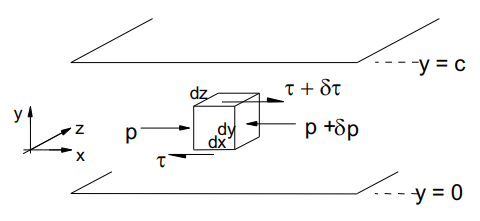
\includegraphics[scale=0.5]{flow_between_planes.png}
        \caption{Flow between planes}
    \end{figure}
    Since the flow is steady we know there is no acceleration so the net force is 0.
    \[0 = p(\delta y\delta z) - (p + \delta p)(\delta y\delta z) + (\tau + \delta \tau)(\delta x\delta z) - \tau(\delta x\delta z)\]
    \[\implies \delta \tau\delta x = \delta p\delta y\]
    \[\implies\pdv{\tau}{y} = \pdv{p}{x}\]
    By definition:
    \[\tau = \mu\pdv{u}{y}\]
    \[\implies\pdv[2]{u}{y} = \frac{1}{\mu}\pdv{p}{x}\]
    \[\int \pdv[2]{u}{y}\,dy = \frac{1}{\mu}\pdv{p}{x}\int dy\]
    \[\pdv{u}{y} = \frac{1}{\mu}\pdv{p}{x}y + A\]
    \[\int \pdv{u}{y}\,dy = \int \frac{1}{\mu}\pdv{p}{x} + A\,dy\]
    \[u = \frac{1}{\mu}\pdv{p}{x}\frac{y^2}{2} + Ay + B\]
    Boundary conditions: no-slip at the walls so \(u = 0\) for \(y = 0, c\)
    \[0 = \frac{1}{\mu}\pdv{p}{x}\frac{0^2}{2} + A\cdot0 + B\implies B = 0\]
    \[0 = \frac{1}{\mu}\pdv{p}{x}\frac{c^2}{2} + Ac\]
    \[\implies A = -\frac{1}{\mu}\pdv{p}{x}\frac{c}{2}\]
    \[\implies u = \frac{1}{2\mu}\pdv{p}{x}(y^2 - yc)\]
    For a long channel, length \(L\) with pressure drop \(\Delta p\) we can approximate
    \[\pdv{p}{x}\approx -\frac{\Delta p}{L}\]
    note that this is negative as by convention in pipes we consider pressure drops which we define as positive
    \[u \approx \frac{1}{2\mu}\frac{\Delta p}{L}(yc - y^2)\]
    This gives a parabolic velocity profile.
    This is known as Poiseuille flow.
    \subsection{Flow in a Circular Pipe}

    \begin{figure}
        \centering
        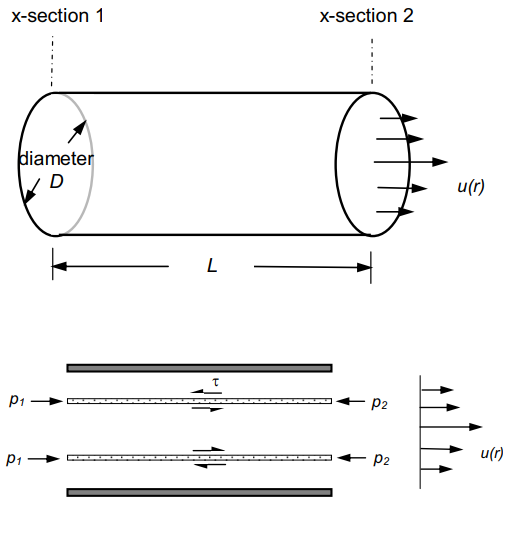
\includegraphics[scale=0.7]{flow_in_circular_pipe.png}
        \caption{Flow in a circular pipe}
    \end{figure}
    Using similar logic to the previous section we can show that:
    \[u(r) = \frac{-(p_2 - p_1)R^2}{4L\mu}\left(1 - \frac{r^2}{R^2}\right)\]
    where \(R\) is the radius of the pipe.
    We can integrate over the circular cross section of a small part of the flow where \(dA = 2\pi rdr\) from \(r = 0\) to \(r = R\). 
    This gives
    \[Q\bar u = \frac{-(p_2 - p_1)\pi R^4}{8L\mu}\]
    \[\implies \bar u = \frac{Q}{A} = \frac{Q}{\pi R^2} = \frac{-(p_2 - p_1)R^2}{8L\mu}\]
    If we rearrange for pressure loss \(\Delta p\) then we get
    \begin{equation}\label{eqn:hagen-poiseuille}
        \Delta p = \frac{128\mu L Q}{\pi D^4} = \frac{32\mu L\bar u}{D^2}
    \end{equation}
    this is the Hagen-Poiseuille equation.
    \subsection{Turbulent Pipe Flow}
    This doesn't work for turbulent flow as we don't consider any forces due to fluid flow \emph{not} in the positive \(x\) direction.
    It is possible to come up with a semi-analytical, semi-empirical formula for frictional head loss \(\Delta H_f\), that is loss due to viscosity and friction.
    This equation is Darcy's equation:
    \begin{equation}\label{eqn:darcy}
        \Delta H_f = \frac{2c_fL\bar u^2}{gD}
    \end{equation}
    Assuming that \(c_f\) depends on \(u\), \(D\), \(\rho\), \(\mu\) and \(k\) where \(k\) is the pipe roughness, it is a measure of average bump size so \([k] = L\). 
    We can use dimensional analysis of \(c_f = c_f(u, D, \rho, \mu, k)\) to find that \(c_f = c_f(Re, k/D)\) where \(k/D\) is the dimensionless (or relative) pipe roughness.
    A quick sanity check of this is that the \(Re\) term takes into account how important viscous forces are and the \(k/D\) term takes into account friction with the walls of the pipe.
    Note that \(k/D\) is bigger for narrower pipes which makes sense as a larger proportion of the fluid is in contact with the walls so their roughness has a larger effect.
    
    \section{Turbulent Flow and Energy Losses}
    It is possible to experimentally measure \(c_f\) as a function of \(Re\) for different values of \(k/D\).
    If we do this then we get something called a Moody chart, shown in figure \ref{fig:moody chart}.
    \begin{figure}[ht]
        \centering
        \begin{tikzpicture}
            \node[opacity=1] at (0, 0) {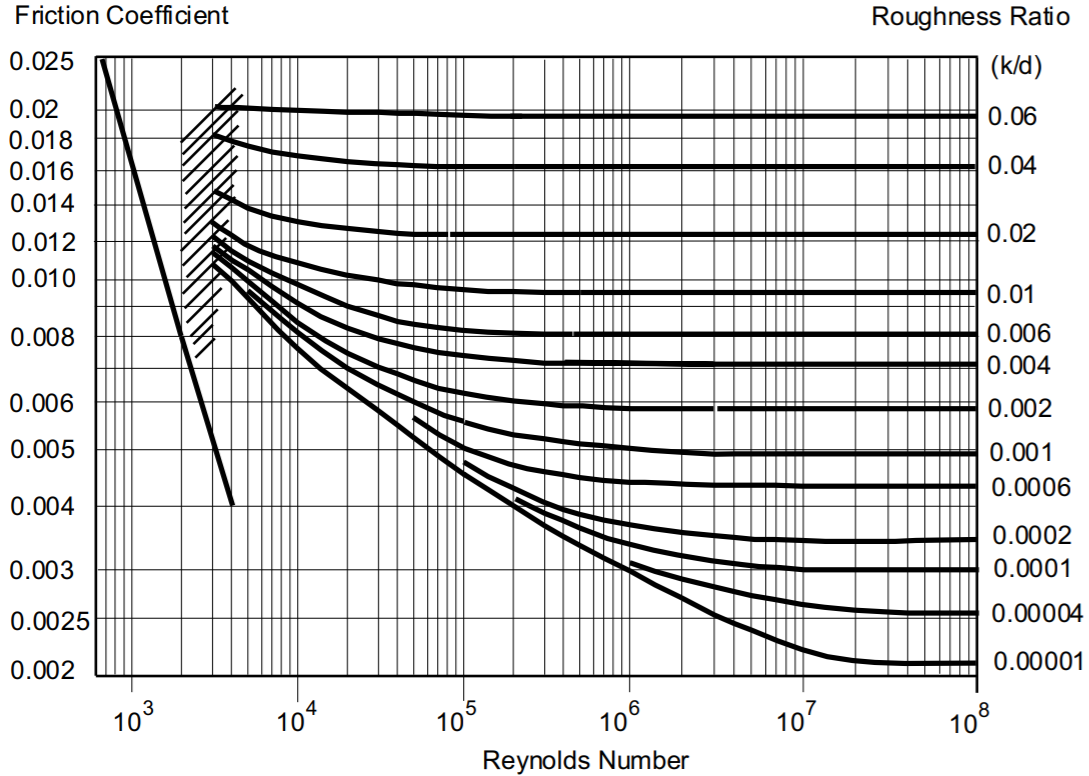
\includegraphics[scale=0.5]{moody_chart.png}};
            %\draw[lightgray] (-5, -5) grid (5, 5);
            \draw[dashed] (4.5, -3.8) -- (-4, 4);
        \end{tikzpicture}
        \caption{Moody chart}
        \label{fig:moody chart}
    \end{figure}
    This chart has several sections. 
    At Reynold's numbers less than 2000 the flow is laminar and we can use equation \ref{eqn:hagen-poiseuille}.
    For Reynold's numbers between 2000 and 4000 the flow is on the boundary between laminar and turbulent and you should use whatever is the worst case scenario for the problem.
    Above 4000 the flow is turbulent.
    Above the dotted line we are in what is known as fully developed or complete turbulence, here increasing Reynold's number has little or no effect on the friction coefficient.
    
    We can compare the linear part with equation \ref{eqn:hagen-poiseuille} and we see that
    \[c_f = \frac{16}{Re}\]
    We can also fit curves to the turbulent section.
    The best of these fits requires an iterative method but a fit that works well enough for most purposes is
    \[c_f = \num{1.38e-3}\left(1 + \left(\num{2e4}\frac{k}{D} + \frac{10^6}{Re}\right)^{1/3}\right)\]
    It is best to use both the formula and the graph to find a value of \(c_f\) and check that they are similar and then use either value or their average.
    
    \subsection{Energy Loss}
    We can quantify energy losses using Bernoulli:
    \[\frac{\bar u_1^2}{2} + \frac{p_1}{\rho} + gz_1 - \left(\frac{\bar u_2^2}{2} + \frac{p_2}{\rho} + gz_2\right) = \Delta E\]
    \[\frac{\rho\bar u_1^2}{2} + p_1 + \rho gz_1 - \left(\frac{\bar u_2^2}{2} + \frac{p_2}{\rho} + \rho gz_2\right) = \Delta p\]
    \[\frac{\bar u_1^2}{2g} + \frac{p_1}{\rho g} + z_1 - \left(\frac{\bar u_2^2}{2} + \frac{p_2}{\rho} + z_2\right) = \Delta H\]
    where \(\Delta E\), \(\Delta p\) and \(\Delta H\) are defined as losses so are positive if the relative value decreases.
    Comparing the equation for head loss with Darcy (equation \ref{eqn:darcy}) we get
    \[\Delta H = \frac{2c_fL\bar u^2}{gD}\implies \frac{4c_fL}{D}\frac{\bar u^2}{2g} = K\frac{\bar u^2}{2g}\]
    For a straight pipe \(K = 4c_fL/D\). 
    \(K\) is the loss coefficient, it is the proportion of head that is lost.
    \(K\) is dimensionless and not to be confused with pipe roughness \(k\) which has dimensions of length.
    
    A pipe normal to the edge of the water can have a variety of values of \(K\).
    If the entrance of the pipe is a right angle then \(K\approx 0.34\).
    If instead the entrance is rounded then \(K\) could be as low as 0.04.
    The reason for the difference is the amount of separation, and therefore energy loss, that occurs.
    
    For a sudden change in pipe cross sectional area from \(A_1\) to \(A_2\) if \(A_1 < A_2\) (ie the pipe gets wider) then
    \[\Delta H = \frac{\bar u^2}{2g}\left(1 - \frac{A_1}{A_2}\right)^2\]
    where \(K = (1 - A_1/A_2)^2\).
    A pipe exit is a special case of as \(A_2\to\infty\) so \(K = 1\).
    This is what we would expect for a pipe exit.
    If instead \(A_1 > A_2\) (ie the pipe contracts) then \(K\) decreases from 0.41 to 0.14 as \(A_2/A_1\) increases fro 0.1 to 0.7.
    On the formula sheet an approximate value of \(K = 0.25\) is given for contraction, this is good enough for most values of \(A_2/A_1\).
    
    \section{More Flow in Pipes}
    \begin{table}[ht]
        \centering
        \begin{tabular}{c|c}
            Pipe & Loss Coefficient\\ \hline
            Radiused \SI{45}{\SIUnitSymbolDegree} & 0.3\\
            Radiused \SI{90}{\SIUnitSymbolDegree} & 0.74\\
            Angular \SI{90}{\SIUnitSymbolDegree} & 1.3
        \end{tabular}
        \caption{Loss coefficients for various pipes}
        \label{tab:loss coefficients}
    \end{table}
    Table \ref{tab:loss coefficients} shows the loss coefficients for some common pipe bends.
    
    \subsection{Pumps}
    A pump supplies head.
    The head supplied varies with Q.
    For a pump \(\Delta H<0\) since \(\Delta H\) is defined as positive head drop so an increase in head must be negative.
    In general the supplied head \(\Delta H_\text{supplied}\) varies with flow rate \(Q\) according to
    \[\Delta H_\text{supplied} = A - BQ^2\]
    for constants \(A\) and \(B\).
    This is shown in figure \ref{fig:pump head}
    
    \begin{figure}[ht]
        \centering
        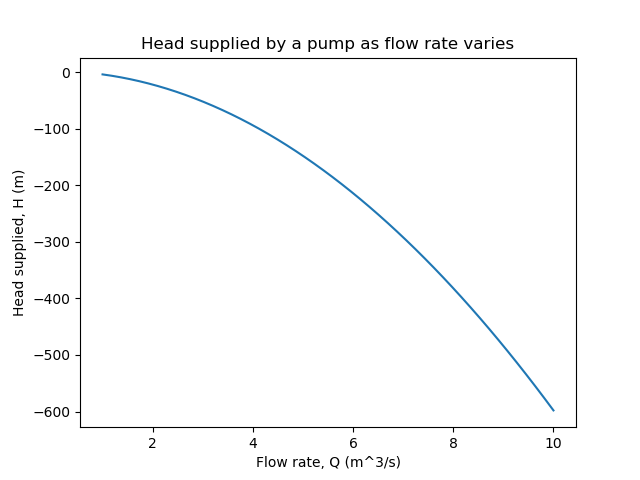
\includegraphics[scale=0.5]{pump_head.png}
        \caption{Head supplied by a pump as flow rate varies}
        \label{fig:pump head}
    \end{figure}

    If all pipes in a system have the same pipe diameter then \(Q\) and \(A\) are constant so \(\bar u = Q/A\) is constant so \(\bar u^2/2g\) is constant.
    This means we can just add the loss coefficients for the different sections of the system.
    If the diameter isn't constant then we need to sum the individual head losses for each section.
    
    The power loss is the energy loss per unit time which is the energy loss per unit volume times the volume per unit time which is
    \[P = \Delta PQ = \rho g\Delta HQ\]
    confusingly \(P\) is power loss but \(\Delta P\) is pressure drop despite both being capital \(P\) and both actually being losses as opposed to total amounts.
    
    \section{Momentum}
    A control volume is an imaginary box surrounding an interesting part of a system.
    All fluid jets entering or leaving a control volume should be normal to the boundary although we often don't draw it as such.
    We make measurements only at the faces of the control volume and we can deduce information from the laws of physics without having to consider what happens inside the control volume.
    
    One such law is Newton's second law:
    \[\vv F = \dv{\vv p}{t}\]
    By considering mass flow rates in \(\dot m_\text{inlet}\) and out \(\dot m_\text{exit}\) of the control volume and also the velocities of these we get
    \[\vv F = \dot m_\text{exit}\vv v_\text{exit} - \dot m_\text{inlet}\vv v_\text{inlet}\]
    often \(\dot m_\text{exit} = \dot m_\text{inlet} = \dot m\) so we can write
    \[\vv F = \dot m\Delta \vv v\]
    There are generally three types of fluid forces:
    \begin{enumerate}
        \item \(\vv F_B\) - Force due to solid boundaries causing a change in velocity
        \item \(\vv F_G\) - Force due to gravity
        \item \(\vv F_P\) - Force due to pressure changes on the sides of the control volume
    \end{enumerate}
    This gives us
    \[\vv F_B + \vv F_G + \vv F_P = \dot m\Delta \vv v\]
    There is a suggested way to solve problems involving changes in momentum.
    It is
    \begin{enumerate}
        \item Draw a control volume around the system
        \item Define the coordinate system
        \item Draw the boundary forces on in the coordinate directions
        \item Calculate the pressure forces at the faces of the control volume
        \item Calculate the force due to gravity on the fluid in the control volume
        \item Calculate the boundary force from the momentum change and other forces
        \item Calculate the reaction force \(\vv R\) due to the boundary force. \(\vv R = -\vv F_B\) by Newton's third law
    \end{enumerate}
    
    \example
    \begin{figure}[ht]
        \centering
        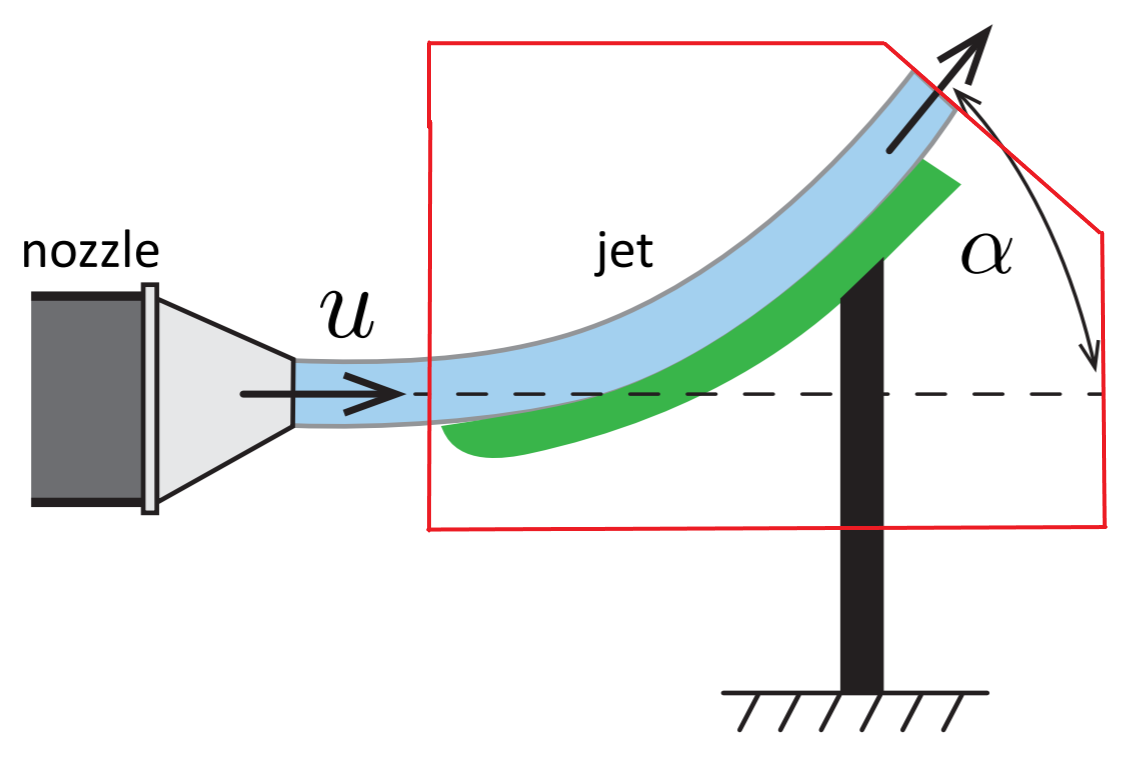
\includegraphics[scale=0.2]{jet_hits_vane_2D_flow.png}
        \caption{Fluid jet hitting a fixed vane}
        \label{fig:jet hits fixed vane 2D flow}
    \end{figure}
    Figure \ref{fig:jet hits fixed vane 2D flow} shows a jet hitting a fixed vane and being deflected.
    What is the resultant force on the vane?
    
    Assumptions:
    \begin{itemize}
        \item Incompressible, steady, 2D flow
        \item Negligible gravitational effects (as the change in height is small)
        \item Atmospheric Pressure throughout
        \item No energy losses
    \end{itemize}
    The control volume is drawn on figure \ref{fig:jet hits fixed vane 2D flow}.
    We take the coordinate system of \(x\) increasing to the right and \(y\) increasing upwards.
    Atmospheric pressure therefore \(\vv F_P = \vv 0\).
    Gravity is negligible therefore \(\vv F_G = \vv 0\).
    This leaves us with
    \[\vv F_B = \dot m\Delta\vv v\]
    All terms in Bernoulli apart from speed cancel so the fluid must exit the control volume at speed \(u\).
    We can split the force equation into
    \[F_{Bx} = \dot m\Delta v_x = \dot m(u\cos\alpha - u) = \dot mu(\cos\alpha - 1)\]
    \[F_{By} = \dot m\Delta v_y = \dot m(u\sin\alpha - 0) = \dot mu\sin\alpha\]
    By continuity \(Q_1 = Q_2\implies u_1A_1 = u_2A_2\implies A_1 = A_2\).
    \[F_{Bx} = \rho Au^2(\cos\alpha - 1)\]
    \[F_{By} = \rho Au^2\sin\alpha\]
    The reaction force has components:
    \[R_x = -\rho Au^2(\cos\alpha - 1) = \rho Au^2(1 - \cos\alpha)\]
    \[R_y = -\rho Au^2\sin\alpha\]
    
    \section{Jets Hitting Vanes}
    A fluid jet hits a flat, circular, fixed plate as shown in figure \ref{fig:circular vane}
    \begin{figure}
        \centering
        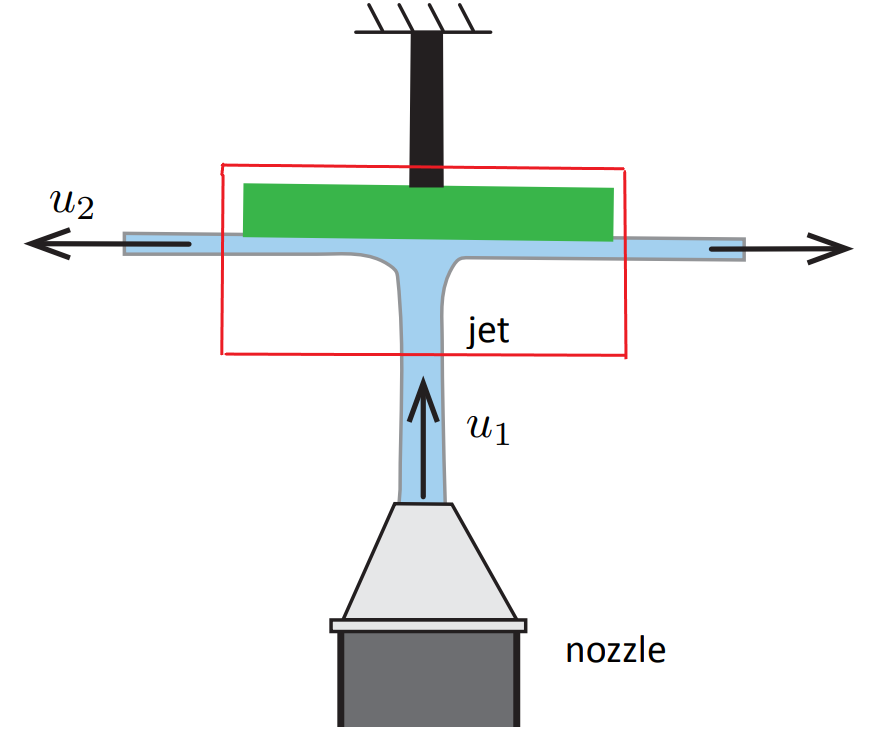
\includegraphics[scale=0.2]{circular_vane.png}
        \caption{A fluid jet hitting a circular vane}
        \label{fig:circular vane}
    \end{figure}
    Assumptions: Radial flow at exit of the control volume, steady, incompressible, 3D flow, no gravitational effects, atmospheric pressure throughout, no energy losses.
    
    The control volume is going to be a cylinder since all jets leave it normal to the boundary.
    We define the \(y\) direction as up and the \(r\) direction as out from the centre since the problem is radially symmetric.
    From our assumptions \(\vv F_P = \vv F_G = \vv 0\).
    This leaves us with
    \[\vv F_B = \dot m\Delta \vv v\]
    \[F_{By} = -u_1\dot m = -\rho A_1u_1^2\]
    \(F_{Br} = 0\) since the radial symmetry causes all forces in the \(r\) direction to cancel.
    Hence \(R_{y} = \rho A_1u_1^2\) and \(R_{r} = 0\).
    This gives a reaction force of \(\vv R = \rho A_1u_1^2 \vh y\).
    
    We can modify the problem above so that the jet is caused to curve down so it follows a path at angle \(\alpha\) to the vertical.
    This means that the fluid exiting the control volume has a \(y\) component to its velocity.
    This gives
    \[F_{By} = \rho A_1u_1(-u_2\cos(180 - \alpha) - u_1)\]
    \[F_{By} = \rho A_1u_1(u_2\cos(\alpha) - u_1)\]
    By Bernoulli we can see \(u_1 = u_2 = u\) since all other terms cancel.
    This gives \(R_y = \rho A u^2(\cos \alpha - 1)\).
    Which gives us a \(y\) component of \(R_y = \rho A u^2(1 - \cos \alpha)\)
    
    We can see that the first case of the flat plate is just a special case of \(\alpha = \SI{90}{\SIUnitSymbolDegree}\).
    The reaction force is maximised at \(\alpha = \SI{180}{\SIUnitSymbolDegree}\) to a value of \(R_y = 2\rho A_1u^2\), this is useful if we are building something like a turbine where we want to maximise the force given to the turbine by a jet.
    
    A jet hits a smooth, vertical wall.
    The angle between the jet and the wall is \(\alpha\).
    Making the same assumptions as before but also assuming 2D flow what is the reaction force on the wall?
    From the assumptions \(\vv F_P = \vv F_G = \vv 0\implies \vv F_B = \dot m\Delta\vv v\).
    \[F_{Bx} = \dot m(0 - u_1\sin\alpha) = \rho A_1 u_1^2\sin\alpha\]
    \(F_{By} = 0\) as the wall is smooth so there is no way for the jet to impart any vertical force on the wall.
    \[\vv R = \rho A_1u_1^2\sin\alpha \vh x\]
    
    
\end{document}
